\documentclass{article}
\usepackage{preprint}
% T1 encoding is needed for accented author names in the bibliography (e.g., \k{e})
\usepackage[T1]{fontenc}

\usepackage{amsmath,amssymb,amsthm,mathtools,bm}
\usepackage{booktabs}
\usepackage{multirow}
\usepackage{graphicx}
\usepackage{xcolor}
\usepackage{float}
\usepackage{tikz}
\usetikzlibrary{arrows.meta}
\usepackage{algorithm}
\usepackage[noend]{algpseudocode}
% Appendix floats use [!htbp] so that LaTeX fills pages itself; \FloatBarrier at section boundaries
% keeps floats from drifting into the next section and avoids the blank pages caused by [H]
\usepackage[section]{placeins}
\renewcommand{\bottomfraction}{0.8}
\renewcommand{\floatpagefraction}{0.85}
\setcounter{topnumber}{4}
\setcounter{bottomnumber}{3}
\setcounter{totalnumber}{6}
% Stack floats from the top of float pages instead of spreading them out vertically
\makeatletter
\setlength{\@fptop}{0pt}
\setlength{\@fpsep}{\floatsep}
\setlength{\@fpbot}{0pt plus 1fil}
\makeatother

% hyperref must come after float-related packages to avoid duplicate anchors
\usepackage{hyperref}
\usepackage{url}

% -------- theorem environments --------
\theoremstyle{plain}
\newtheorem{theorem}{Theorem}[section]
\newtheorem{lemma}[theorem]{Lemma}
\newtheorem{corollary}[theorem]{Corollary}
\newtheorem{proposition}[theorem]{Proposition}
\theoremstyle{remark}
\newtheorem{remark}[theorem]{Remark}

% -------- notation --------
\newcommand{\Expl}{\mathrm{Expl}}
\newcommand{\Proj}{\Pi}
\newcommand{\simplex}{\Delta}
% Vectors are bold lowercase
\newcommand{\bx}{{\bm{x}}}
\newcommand{\by}{{\bm{y}}}
\newcommand{\bv}{{\bm{v}}}
\newcommand{\bw}{{\bm{w}}}
\newcommand{\bz}{{\bm{z}}}
\newcommand{\bu}{{\bm{u}}}
\newcommand{\bg}{{\bm{g}}}
\newcommand{\bq}{{\bm{q}}}
\newcommand{\br}{{\bm{r}}}
\newcommand{\be}{{\bm{e}}}
\newcommand{\brho}{{\bm{\rho}}}
\newcommand{\bell}{{\bm{\ell}}}
\newcommand{\aug}{\tilde{\bell}}
% Nash strategy, step of the learner, self-play vertex and self-play weight
\newcommand{\xs}{\bx^{\star}}
\newcommand{\dx}{{\bm{s}}}
\newcommand{\esp}{\be_{\mathrm{sp}}}
\newcommand{\wsp}{w_{\mathrm{sp}}}
\newcommand{\coda}{CoDA}
\newcommand{\codar}{CoDA-R}
\newcommand{\rnad}{R-NaD-PPO}

% -------- labels of the overview figure (figures/overview.tex) --------
\newcommand{\ovLearner}{Learner}
\newcommand{\ovPool}{Pool of frozen opponents}
\newcommand{\ovOracle}{Oracle\\(optional)}
\newcommand{\ovWeightRule}{Weight rule}
\newcommand{\ovPolicyUpdate}{Policy update}
\newcommand{\ovUpdateText}{regularized step against\\itself and the weighted pool}
\newcommand{\ovLossRates}{loss rates}
\newcommand{\ovWeights}{weights}
\newcommand{\ovGames}{games}
\newcommand{\ovExploiter}{exploiter}
\newcommand{\ovSelfPlay}{self-play}
\newcommand{\ovThreshold}{threshold}

\title{Coupled Dual-Adversarial Regularized Self-Play}

\author{YuLiang Xu}
\affiliation{Beijing No.~8 High School}
\email{ganggang2011@icloud.com}

\begin{document}

\maketitle

\begin{abstract}
Self-play for two-player zero-sum games can cycle when strategies beat one another in a rock--paper--scissors pattern. Regularized self-play removes the cycles and trains a single network, but that network only ever plays itself and cannot learn from external opponents. Population methods train against a pool of opponents, but what they guarantee to converge is a mixture over the pool, and the network being trained has no guarantee. We propose Coupled Dual-Adversarial Regularized self-play (CoDA-R), which trains one network against itself and against a pool. Before each regularized policy update, a closed-form rule gives training weight only to the pool opponents that currently beat the network, according to their lead. For the exact algorithm, we prove that the trained policy itself converges to a Nash equilibrium however opponents enter or leave the pool, and that an approximate best response in the pool guarantees progress toward equilibrium at every step, proportional to the squared exploitability. We implement CoDA-R on proximal policy optimization (PPO) and compare it, at a matched budget, with baselines tuned by the same protocol on five imperfect-information games. CoDA-R reaches the lowest exploitability among single-network methods on three games, 73\% and 36\% below the regularized self-play baseline on Goofspiel and Leduc poker, ties the best on one, and is second on one. Controlled experiments show that the pool repairs vulnerabilities that self-play almost never reaches and keeps a near-equilibrium network from drifting away.
\end{abstract}

% ----------------------------------------------------------------------
\section{Introduction}
% ----------------------------------------------------------------------

Two-player zero-sum games are the basic model of adversarial decision making. Board games, poker, and real-time strategy games are direct instances~\citep{silver2018alphazero,brown2018libratus,vinyals2019alphastar,perolat2022stratego}, and the training objectives of generative adversarial networks and robust optimization are also min--max problems~\citep{goodfellow2014gan,daskalakis2018optimism}. The natural solution concept is a Nash strategy, which in a symmetric game is a strategy that no opponent beats in expectation. The common way to find one is self-play: the current policy plays against itself or its past versions and is updated by reinforcement learning, with neither human data nor an explicit opponent model.

Self-play has a well-known failure mode. Real games contain nontransitive cycles~\citep{czarnecki2020spinning}, in which a first strategy beats a second, the second beats a third, and the third beats the first. Naive self-play, which only updates against the current policy, chases these cycles and does not converge~\citep{balduzzi2018mechanics,balduzzi2019openended}. Two families of remedies exist. \emph{Regularized self-play}, such as Regularized Nash Dynamics (R-NaD) and Magnetic Mirror Descent (MMD), penalizes the distance between the policy and a reference policy that is moved periodically. This turns the cycling into convergence, and the guarantee holds for the single network being trained~\citep{perolat2021rnad,perolat2022stratego,sokota2023mmd}. But the network only plays itself. Scripted opponents, earlier snapshots, and \emph{exploiters}, i.e., opponents trained specifically to beat the current policy, cannot be used, so vulnerabilities that self-play does not reach are neither found nor repaired~\citep{openai2019dota,bansal2018emergent}. \emph{Population methods}, such as Double Oracle, Policy-Space Response Oracles (PSRO), prioritized fictitious self-play (PFSP), and league training, train against a pool of such opponents~\citep{mcmahan2003doubleoracle,lanctot2017psro,vinyals2019alphastar}. Where they have a guarantee, it holds for a mixture over the pool members or for a separately learned average network, and the network being trained has none. Rules that weight pool opponents by win rate, such as PFSP and the sampler of OpenAI Five, have no convergence proof.

\begin{figure}[t]
\begin{center}
% Overview figure shared by main.tex and main_zh.tex; the including file defines the \ov... label macros
\resizebox{0.98\linewidth}{!}{%
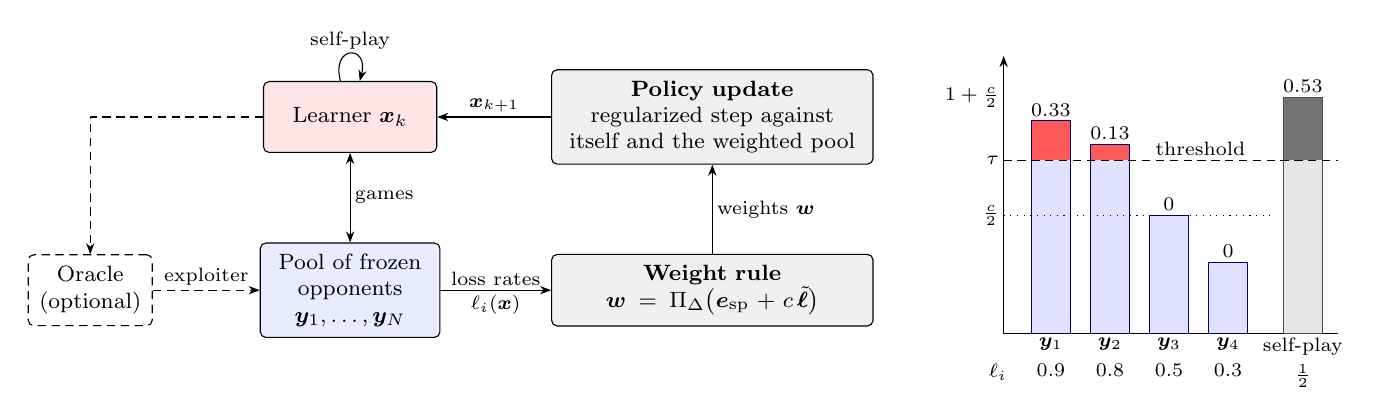
\begin{tikzpicture}[font=\footnotesize, >={Stealth[length=4pt]},
  box/.style={draw, rounded corners=2pt, align=center, inner sep=4pt, minimum height=9mm},
  note/.style={font=\scriptsize, align=center, inner sep=1.5pt}]
% -------- left panel: one step --------
\node[box, minimum width=22mm, fill=red!10] (learner) at (0,0) {\ovLearner\ $\bx_k$};
\node[box, text width=20mm, fill=blue!8] (pool) at (0,-2.2) {\ovPool\\$\by_1,\dots,\by_N$};
\node[box, densely dashed, minimum width=14mm] (oracle) at (-3.3,-2.2) {\ovOracle};
\node[box, text width=38mm, fill=black!6] (dual) at (4.6,-2.2) {\textbf{\ovWeightRule}\\$\bw=\Proj_{\simplex}\big(\esp+c\,\aug\big)$};
\node[box, text width=38mm, fill=black!6] (primal) at (4.6,0) {\textbf{\ovPolicyUpdate}\\\ovUpdateText};
\path[->] (learner) edge[loop above, looseness=5] node[note, above] {\ovSelfPlay} (learner);
\draw[<->] (learner) -- node[note, right] {\ovGames} (pool);
\draw[->] (pool) -- node[note, above] {\ovLossRates} node[note, below] {$\ell_i(\bx)$} (dual);
\draw[->] (dual) -- node[note, right] {\ovWeights\ $\bw$} (primal);
\draw[->] (primal) -- node[note, above] {$\bx_{k+1}$} (learner);
\draw[->, densely dashed] (oracle) -- node[note, above] {\ovExploiter} (pool);
\draw[->, densely dashed] (learner.west) -| (oracle.north);
% -------- right panel: the weight rule as a threshold, c = 2 and loss rates 0.9, 0.8, 0.5, 0.3 --------
\begin{scope}[shift={(8.3,-2.75)}, y=1.5cm]
\def\tauv{1.4667}
\draw[->] (0,0) -- (0,2.35);
\draw (0,0) -- (4.25,0);
% pool members: position, height c * loss rate, index, loss rate
\foreach \xpos/\h/\lab/\lr in {0.35/1.8/1/0.9, 1.1/1.6/2/0.8, 1.85/1.0/3/0.5, 2.6/0.6/4/0.3} {
  \fill[blue!12] (\xpos,0) rectangle (\xpos+0.5,\h);
  \draw[blue!45!black] (\xpos,0) rectangle (\xpos+0.5,\h);
  \node[note, below] at (\xpos+0.25,0) {$\by_{\lab}$};
  \node[note, below] at (\xpos+0.25,-0.22) {\lr};
}
% the part above the threshold is the weight
\foreach \xpos/\h/\wt in {0.35/1.8/0.33, 1.1/1.6/0.13} {
  \fill[red!65] (\xpos,\tauv) rectangle (\xpos+0.5,\h);
  \draw[blue!45!black] (\xpos,0) rectangle (\xpos+0.5,\h);
  \node[note, above] at (\xpos+0.25,\h) {\wt};
}
\node[note, above] at (2.1,1.0) {0};
\node[note, above] at (2.85,0.6) {0};
% self-play arm with height 1 + c / 2
\fill[black!10] (3.55,0) rectangle (4.05,2.0);
\fill[black!55] (3.55,\tauv) rectangle (4.05,2.0);
\draw[black!70] (3.55,0) rectangle (4.05,2.0);
\node[note, above] at (3.8,2.0) {0.53};
\node[note, below] at (3.8,0) {\ovSelfPlay};
\node[note, below] at (3.8,-0.22) {$\tfrac12$};
\node[note, below left] at (0.1,-0.22) {$\ell_i$};
% threshold and tie level
\draw[densely dashed] (0,\tauv) -- (4.25,\tauv);
\node[note, above] at (2.5,\tauv) {\ovThreshold};
\draw[dotted] (0,1.0) -- (3.4,1.0);
\node[note, left] at (0,1.0) {$\tfrac c2$};
\node[note, left] at (0,2.0) {$1+\tfrac c2$};
\node[note, left] at (0,\tauv) {$\tau$};
\end{scope}
\end{tikzpicture}%
}

\end{center}
\vspace{-4pt}
\caption{One step of \codar{}. Left: the learner plays the pool and itself; the weight rule turns its loss rates into weights, and the policy update takes a regularized step against the weighted opponents. Right: the weight rule as a threshold (here $c=2$). Pool member $i$ has height $c\,\ell_i$ and self-play has height $1+\tfrac c2$; the part above the threshold $\tau$ is the weight, so members that tie or lose get exactly zero.}
\label{fig:overview}
\end{figure}

This paper asks whether one network can train against an open pool of opponents and still be the object that converges. We propose Coupled Dual-Adversarial Regularized self-play (\codar{}), for which the answer is yes when its steps are computed exactly. \codar{} keeps a single policy, the \emph{learner}, and a pool of frozen opponents, and each step has two parts (Figure~\ref{fig:overview}). First, a closed-form rule assigns training weights. A pool opponent receives weight only if it currently beats the learner, and more weight for a larger lead; opponents that tie or lose receive exactly zero, and the remaining weight goes to self-play. Second, the learner takes a regularized step against itself and the weighted pool, as in regularized self-play. The weights play the role of an adversary's dual variable, since they are chosen to maximize the learner's weighted loss, which gives the method its name. The rule needs only the learner's loss rate against each pool member, which is estimated from the training games themselves. Any agent that can play the game can therefore be a pool member, including scripted bots, agents of other architectures, and exploiters produced by an \emph{oracle} during training, whereas PSRO needs the payoffs between all pairs of pool members.

The two parts are coupled by one inequality (Theorem~\ref{thm:energy}). Every step of the learner and every unit of weight held by the pool is paid for by a decrease of the squared distance between the learner and a Nash strategy. This distance is finite, so the steps and the pool weights must both vanish, and a policy that has stopped moving while no pool member holds weight is a Nash strategy of the full game. The argument holds for any pool contents and any schedule of changes to the pool. The same inequality shows what the pool adds: when the pool contains an approximate best response to the learner, each step moves the learner toward equilibrium by an amount proportional to its squared exploitability (Theorem~\ref{thm:oracle}). Our contributions are as follows.
\begin{itemize}
\item \textbf{Algorithm.} \codar{} trains a single network against itself and an open pool of black-box opponents, with a closed-form weight rule that carries no state between steps. Prior pool methods guarantee a mixture or a time average, and regularized self-play admits no external opponents; \codar{} admits any opponent and keeps the guarantee on the trained policy itself. It wraps an unmodified PPO learner and adds only a proximal reward term (\S\ref{sec:alg}, \S\ref{sec:impl}).
\item \textbf{Theory.} A single energy inequality charges both policy movement and pool weight to the distance to a Nash equilibrium. It yields last-iterate convergence of the trained policy for any sequence of pool changes, an $O(K^{-1/4})$ last-iterate rate once the pool stops changing, bounds on exploitability in terms of quantities observed during training, and versions of all bounds with errors (\S\ref{sec:theory}). When the pool contains an approximate best response, it also bounds the progress of each step from below by the squared exploitability (Theorem~\ref{thm:oracle}).
\item \textbf{Experiments.} In about $10^8$ per-step records of the exact algorithm, no inequality is violated. With PPO, at a matched budget and with every baseline tuned by the same protocol, the \codar{} learner has the lowest tail exploitability among single networks on Goofspiel(4), Leduc poker, and 3$\times$3 abrupt Dark Hex, and ties \rnad{} on abrupt Phantom Tic-Tac-Toe. Controlled experiments isolate what the pool contributes and where the weight rule differs from PFSP (\S\ref{sec:exp}).
\end{itemize}
The reference point of the weight rule is fixed at pure self-play. A variant in which it moves with training, the natural design for solving the game restricted to the pool, gets stuck at non-equilibrium points; \S\ref{sec:coda} gives a counterexample and explains why the reference point must be fixed.

% ----------------------------------------------------------------------
\section{Problem Setting}
\label{sec:prelim}
% ----------------------------------------------------------------------

\subsection{Games, Loss Rates, and Exploitability}

We consider a finite two-player zero-sum game in which the two seats are assigned at random before each game. The game is then \emph{symmetric}, i.e., both players face the same decision problem, and any finite two-player zero-sum game becomes symmetric in this way. A player has $M$ pure strategies (deterministic policies), and a mixed strategy is a probability distribution over them, i.e., a point of the probability simplex
\[
X=\simplex_M:=\Big\{\bx\in\mathbb R^M:\ x_i\ge0,\ \textstyle\sum_ix_i=1\Big\}.
\]
We write $\simplex_n$ for the probability simplex in $\mathbb R^n$ throughout. In a sequential game with perfect recall, mixed strategies are equivalent to the behavior policies that a network represents~\citep{kuhn1953}, so this normal form covers games such as poker with no further assumption. $M$ is then very large, but the algorithm never enumerates pure strategies; the normal form is used only in the analysis.

Let $\ell(\bx;\by)\in[0,1]$ denote the expected loss of strategy $\bx$ against $\by$, with outcomes scaled so that a loss counts 1, a win 0, and a tie $\tfrac12$. We call it the \emph{loss rate}. Zero-sum payoffs and symmetry give $\ell(\bx;\by)+\ell(\by;\bx)=1$, so there exists a skew-symmetric matrix $S=-S^\top$ such that
\[
\ell(\bx;\by)=\tfrac12+\bx^\top S\by,\qquad \bx^\top S\bx=0 .
\]
In particular, every strategy ties with itself. The quality of a strategy is measured by its \emph{exploitability}, the amount by which the best opponent beats it,
\[
\Expl(\bx):=\max_{\by\in X}\ell(\bx;\by)-\tfrac12=\max_j(S^\top \bx)_j\ \ge\ 0 .
\]
A \emph{Nash strategy} $\xs$ is one with $\Expl(\xs)=0$. It exists by the minimax theorem~\citep{vonneumann1928}, and
\begin{equation}
\xs\ \text{is Nash}\iff {\xs}^\top S\by\le0\ \ \forall \by\in X\iff \by^\top S\xs\ge0\ \ \forall \by\in X .
\label{eq:nash}
\end{equation}

\subsection{Learner, Pool, and Oracle}
\label{sec:setting}

The \emph{learner} is the single policy being trained, and $\bx_k$ denotes it after step $k$. Besides playing itself, it can play a \emph{pool} $P=\{\by_1,\dots,\by_N\}\subset X$ of frozen opponents. A pool member can be any agent that plays the game, for example an earlier snapshot of the learner, a scripted bot, an agent with a different architecture, or an exploiter. Members are black boxes. The algorithm uses only the outcomes of games between the learner and each member, summarized by the loss rates
\[
\ell_i(\bx):=\ell(\bx;\by_i)=\tfrac12+(S\by_i)^\top\bx ,\qquad i=1,\dots,N,
\]
each an affine function of $\bx$ with constant gradient $S\by_i$. It uses neither the payoff matrix $S$ nor the payoffs among pool members. The pool may change between steps. An \emph{oracle} is any procedure that, given the frozen learner, returns an opponent meant to beat it, for example an exploiter trained by reinforcement learning or, in small games, an exact best response; its output is added to the pool.

The goal is that the learner itself becomes unexploitable, $\Expl(\bx_k)\to0$. This is last-iterate convergence of a single network, as opposed to convergence of a mixture over many networks. The pool serves this goal in two ways. It lets opponents that self-play would never produce shape the learner (\S\ref{sec:exp-mech}), and a pool that contains good responses to the learner speeds up convergence (Theorem~\ref{thm:oracle}).

\subsection{Projections}

Throughout, $\|\cdot\|$ denotes the Euclidean norm and $\Proj_C$ the Euclidean projection onto a closed convex set $C$. The projection is characterized by the \emph{projection inequality}
\begin{equation}
\bw=\Proj_C(\bv)\iff(\bv-\bw)^\top(\bu-\bw)\le0\quad\forall \bu\in C ,
\label{eq:obtuse}
\end{equation}
which implies that it is monotone and nonexpansive~\citep{bauschke2011convex}: for $\bw=\Proj_C(\bz)$ and $\bw'=\Proj_C(\bz')$, taking $\bu=\bw'$ and $\bu=\bw$ respectively in \eqref{eq:obtuse} and adding gives
\begin{equation}
(\bz-\bz')^\top(\bw-\bw')\ \ge\ \|\bw-\bw'\|^2\ \ge\ 0 .
\label{eq:monotone}
\end{equation}
The projection onto the simplex has the threshold form $\Proj_{\simplex_n}(\bz)_i=(z_i-\tau)^+$, where $(u)^+:=\max(u,0)$ and the threshold $\tau$ is chosen so that the components sum to one; components below the threshold are exactly zero, and $\tau$ is computed in $O(n\log n)$ time~\citep{duchi2008projection}. The diameter of the simplex is $D=\sqrt2$. Apart from the minimax theorem and the Hartman--Stampacchia theorem, the proofs in this paper use only the projection inequality, completing the square, and the polarization identity $\|\bu+\bv\|^2=\|\bu\|^2+\|\bv\|^2+2\bu^\top\bv$. Table~\ref{tab:notation} collects the notation.

\begin{table}[t]
\caption{Notation.}
\label{tab:notation}
\begin{center}
\small
\begin{tabular}{ll}
\toprule
Symbol & Meaning \\
\midrule
$X=\simplex_M$ & mixed strategies over $M$ pure strategies \\
$\ell(\bx;\by)$, $S$ & loss rate of $\bx$ against $\by$; $\ell(\bx;\by)=\tfrac12+\bx^\top S\by$ with $S=-S^\top$ \\
$\Expl(\bx)$, $\xs$ & exploitability; a Nash strategy, $\Expl(\xs)=0$ \\
$\bx_k$, $\dx_k$ & the learner after step $k$; its step $\dx_k=\bx_{k+1}-\bx_k$ \\
$P=\{\by_1,\dots,\by_N\}$, $\ell_i(\bx)$ & pool of frozen opponents; loss rate of $\bx$ against $\by_i$ \\
$\aug(\bx)$ & $(\ell_1(\bx),\dots,\ell_N(\bx),\tfrac12)$, the loss rates with self-play appended \\
$\bw(\bx)$, $\bw_P$, $\wsp$ & weights; their pool coordinates; the self-play weight \\
$\esp$ & $(0,\dots,0,1)$, all weight on self-play \\
$c$, $\eta$ & dual strength; proximal strength \\
$a$, $b$ & pool weight $1-\wsp$; pool pressure $\sum_iw_i(\ell_i-\tfrac12)$ \\
$\xi_k$, $\delta_k$, $\varepsilon$ & errors of the loss estimates, of the policy update, and of the oracle \\
\bottomrule
\end{tabular}
\end{center}
\end{table}

% ----------------------------------------------------------------------
\section{\codar{}}
\label{sec:alg}
% ----------------------------------------------------------------------

\begin{algorithm}[t]
\caption{One step of \codar{} (exact form; the PPO implementation is described in \S\ref{sec:impl})}
\label{alg:codar}
\begin{algorithmic}[1]
\Require learner $\bx_k$, pool $P=\{\by_1,\dots,\by_N\}$, dual strength $c>0$, proximal strength $\eta>0$
\State $\aug(\bx)\leftarrow\big(\ell_1(\bx),\dots,\ell_N(\bx),\tfrac12\big)$ \Comment{loss rates of the learner; self-play ties}
\State $\bw\leftarrow\Proj_{\simplex_{N+1}}\big(\esp+c\,\aug(\bx)\big)$ \Comment{weight rule (dual side)}
\State Train the learner against itself (coefficient 1) and each $\by_i$ (coefficient $w_i$), with penalty $\tfrac\eta2\|\bx-\bx_k\|^2$ \Comment{policy update (primal side)}
\State $\bx_k\leftarrow\bx_{k+1}$ \Comment{move the policy anchor}
\State Optionally call the oracle on $\bx_{k+1}$ and add the returned opponent to $P$
\end{algorithmic}
\end{algorithm}

\codar{} maintains the learner $\bx_k$ and the pool $P$. One step (Algorithm~\ref{alg:codar}, Figure~\ref{fig:overview}) has two parts. The \emph{weight rule} takes the learner's loss rate against every pool member and assigns weights: members that currently beat the learner receive weight according to their lead, the others receive exactly zero, and the remaining weight goes to self-play. The \emph{policy update} then takes a regularized step for the learner against itself and the weighted pool, staying close to the previous policy $\bx_k$. Since the weights are chosen against the learner, as the maximizing variable of a min--max problem, we also call the weight rule the dual side and the policy update the primal side. In the exact algorithm analyzed in \S\ref{sec:theory}, both parts are evaluated at the new policy $\bx_{k+1}$, i.e., the step is implicit; \S\ref{sec:impl} describes the approximation used with PPO.

\subsection{Weight Rule}
\label{sec:dual}

Self-play is treated as one more opponent, the \emph{self-play arm}. Every strategy ties with itself, so the loss rate of this arm is the constant $\tfrac12$, and the augmented loss vector is
\[
\aug(\bx):=\big(\ell_1(\bx),\dots,\ell_N(\bx),\tfrac12\big)\in\mathbb R^{N+1}.
\]
Let $\esp:=(0,\dots,0,1)\in\simplex_{N+1}$ denote the weight vector of pure self-play, and let $c>0$ be the \emph{dual strength}, which is held fixed during training. Given a policy $\bx$, the weights are
\begin{equation}
\bw(\bx):=\operatorname*{arg\,max}_{\bw\in\simplex_{N+1}}\Big[\bw^\top\aug(\bx)-\frac1{2c}\|\bw-\esp\|^2\Big]=\Proj_{\simplex_{N+1}}\big(\esp+c\,\aug(\bx)\big),
\label{eq:dual}
\end{equation}
where the second equality follows from completing the square. The first term in the brackets moves weight toward the opponents against which the learner loses most, and the second pulls the weights back toward pure self-play, more weakly for larger $c$. We call $\esp$ the \emph{dual anchor}, and we write $\bw_P$ for the pool coordinates of $\bw$ (its first $N$ components) and $\wsp$ for the self-play weight.

By the threshold form of the projection, $w_i=(c\,\ell_i(\bx)-\tau)^+$ for the pool members and $\wsp=(1+\tfrac c2-\tau)^+$ (Figure~\ref{fig:overview}, right). The self-play arm has a head start of 1 over a member that ties, so a member has to lead to rise above the threshold. With a single pool member that leads by $\mu$, i.e., $\ell_1(\bx)=\tfrac12+\mu$, the rule reduces to $w_1=\operatorname{clip}(\tfrac{c\mu}2,0,1)$: no weight without a lead, and above that a weight proportional to the lead, with slope set by $c$. The next lemma states the general properties; its proof is in Appendix~\ref{app:dual}.

\begin{lemma}[Properties of the weight rule]
\label{lem:dual}
(a) $\bw(\bx)=\esp$ if and only if $\max_{i\in P}\ell_i(\bx)\le\tfrac12$.\\
(b) A member holding weight must be currently beating the learner:
\[
w_i(\bx)>0\ \Longrightarrow\ \ell_i(\bx)-\tfrac12\ \ge\ \frac{1-\wsp(\bx)+w_i(\bx)}{c}\ >\ 0 .
\]
(c) If the pool has a single member and $\ell_1(\bx)=\tfrac12+\mu$, then $w_1(\bx)=\operatorname{clip}(\tfrac{c\mu}{2},0,1)$.
\end{lemma}

By (a), when no member beats the learner, all weight goes to self-play and the step is a regularized self-play step, the common skeleton of R-NaD and MMD; \codar{} departs from regularized self-play only while some opponent beats the learner. By (b), a member that holds weight is winning, and heavier members lead by more. With several members the weights share one threshold and have no per-member closed form. For example, $c=4$ and two members with loss rate 0.9 give $\esp+c\,\aug=(3.6,3.6,3)$ and $\bw=(\tfrac12,\tfrac12,0)$, with no weight left for self-play.

The anchor is placed at $\esp$ because the correct weights at the solution are known in advance: no opponent beats a Nash strategy, so by (a) the weights there are $\esp$. Since the anchor is fixed, $\bw(\bx)$ is a continuous closed-form function of the current loss rates and carries no state from earlier steps. A new pool member needs no initialization, and a member regains weight as soon as it wins again. \S\ref{sec:coda} shows that an anchor that moves with training loses the convergence guarantee.

\subsection{Policy Update}
\label{sec:primal}

Fix the previous policy $\bx_k$, which serves as the \emph{policy anchor}, and the \emph{proximal strength} $\eta>0$. Suppose for the moment that the opponents are fixed: a self-play opponent $\bar{\by}$ with coefficient 1 and the pool members with weights $\bw$. The policy update minimizes the weighted loss rate plus a proximal penalty,
\begin{equation}
f_k(\bx):=\ell(\bx;\bar{\by})+\sum_{i\in P}w_i\,\ell_i(\bx)+\frac\eta2\|\bx-\bx_k\|^2,\qquad \bx\in X .
\label{eq:primal-obj}
\end{equation}
With $A:=[S\by_1\cdots S\by_N]\in\mathbb R^{M\times N}$, the gradient of the first two terms is the constant vector $S\bar{\by}+A\bw_P$. Completing the square then gives the minimizer $\Proj_X\big(\bx_k-\tfrac1\eta[S\bar{\by}+A\bw_P]\big)$, a projected step of size $1/\eta$ from $\bx_k$ that lowers the weighted loss rate. The exact algorithm evaluates the opponents at the solution itself, $\bar{\by}=\bx_{k+1}$ and $\bw=\bw(\bx_{k+1})$, so the update is
\begin{equation}
\bx_{k+1}=\Proj_X\Big(\bx_k-\tfrac1\eta\big[S\bx_{k+1}+A\,\bw(\bx_{k+1})_P\big]\Big).
\label{eq:primal}
\end{equation}
The unknown appears on both sides, so the update is implicit. By the projection inequality, \eqref{eq:primal} is equivalent to the variational inequality
\begin{equation*}
\big\langle S\bx_{k+1}+A\,\bw(\bx_{k+1})_P+\eta(\bx_{k+1}-\bx_k),\ \bx'-\bx_{k+1}\big\rangle\ \ge\ 0\qquad\forall \bx'\in X ,
\tag{VI}
\label{eq:P}
\end{equation*}
whose three terms are the gradients at $\bx_{k+1}$ of the three terms of \eqref{eq:primal-obj}: self-play, pool, and proximal penalty. For any $\bx_k$ and any pool, \eqref{eq:P} has exactly one solution (Proposition~\ref{prop:unique} in Appendix~\ref{app:unique}). All later proofs insert a suitable test point $\bx'$ into \eqref{eq:P}. We write
\[
\bv_{k+1}:=\bx_{k+1}+\textstyle\sum_iw_i(\bx_{k+1})\,\by_i,\qquad t_k:=2-\wsp(\bx_{k+1})\ \ge\ 1
\]
for the combined opponent and its total mass. Then $S\bv_{k+1}$ is the sum of the first two terms of \eqref{eq:P}, and \eqref{eq:P} says that the learner makes a proximal best response to $\bv_{k+1}$.

The implicit form matters. The analysis needs the weights and the self-play opponent to be evaluated at the same point $\bx_{k+1}$ (Lemma~\ref{lem:B}). If the self-play opponent is instead the previous policy $\bx_k$, the resulting explicit update drifts away from equilibrium, and its exploitability stalls near 0.1 in our matrix-game runs (Appendix Figure~\ref{fig:theory-nec}).

\subsection{Self-Play Coefficient and Opponent Sampling}
\label{sec:share}

Self-play enters \eqref{eq:P} with coefficient 1 at every step, whatever the self-play weight $\wsp$, so the combined opponent always has mass $t_k\ge1$. The coefficient has to be a positive constant. With coefficient 0, the first two terms of \eqref{eq:P} vanish once the pool weights reach zero, and every $\bx$ is a fixed point. With the coefficient set to the self-play weight $\wsp(\bx_{k+1})$, the self-play term $\wsp(\bx)S\bx$ is no longer skew-symmetric in $\bx$, and the monotonicity behind Proposition~\ref{prop:unique} is lost.

The coefficients describe the training objective, and the sampling probabilities can be chosen separately. An implementation can draw opponents from any distribution $\br$ over the arms and weight each game by the importance ratio of its arm, $1/r_{\mathrm{sp}}$ for self-play and $w_i/r_i$ for member $i$; the expected update is then exactly that of \eqref{eq:P}. We draw opponents from the weights themselves, $\br\propto(\bw_P,\wsp)$, with a floor on the self-play arm that bounds its importance ratio. Sampling in proportion to the coefficients, $\br=(\bw_P,1)/t_k$, would cap the pool's share of the games at $(1-\wsp)/(2-\wsp)\le\tfrac12$ and leave few games for estimating the loss rates of exactly the members that hold weight.

% ----------------------------------------------------------------------
\section{Theoretical Analysis}
\label{sec:theory}
% ----------------------------------------------------------------------

This section analyzes the exact algorithm: every step solves \eqref{eq:P} exactly on the normal form of \S\ref{sec:prelim}, and the pool $P_k$ may change arbitrarily between steps. Table~\ref{tab:guarantees} summarizes the results. \S\ref{sec:energy} proves the inequality on which all of them rest, \S\ref{sec:conv} derives convergence, certificates, and rates, \S\ref{sec:oracle-rate} quantifies what an oracle adds, and \S\ref{sec:inexact} treats mixtures and inexact steps.

\begin{table}[t]
\caption{Guarantees for the exact algorithm. $K$ is the number of steps, and $n$ is the number of most recent steps over which the pool has not changed.}
\label{tab:guarantees}
\begin{center}
\footnotesize
\setlength{\tabcolsep}{4pt}
\begin{tabular}{p{2.3cm}p{5.6cm}p{3.6cm}l}
\toprule
Object & Guarantee & Condition on the pool & Result \\
\midrule
Learner $\bx_k$ & converges to a Nash strategy & any sequence of pools & Theorem~\ref{thm:conv} \\
Learner $\bx_k$ & $\min_{k<K}\Expl(\bx_{k+1})=O(K^{-1/2})$ & any sequence of pools & Theorem~\ref{thm:rate} \\
Learner $\bx_K$ & $\Expl(\bx_K)=O(n^{-1/4})$ & unchanged for $n$ steps & Theorem~\ref{thm:rate} \\
Learner $\bx_{k+1}$ & $\Expl(\bx_{k+1})\le\tfrac12a+\eta D\|\dx_k\|$, observable in training & any pool & Theorem~\ref{thm:cert} \\
Learner $\bx_{k+1}$ & squared distance to every Nash strategy falls by $\tfrac{c}{4\eta}[\Expl(\bx_k)-\varepsilon]^{+2}$ & contains an $\varepsilon$-best response to $\bx_k$ & Theorem~\ref{thm:oracle} \\
Time average $\bar{\bq}_K$ & $\Expl(\bar{\bq}_K)\le\eta/K$ & any sequence of pools & Proposition~\ref{prop:mix} \\
All of the above & same bounds with additive error terms & inexact steps & Theorem~\ref{thm:inexact} \\
\bottomrule
\end{tabular}
\end{center}
\end{table}

\subsection{Energy Inequality}
\label{sec:energy}

Fix a step $k$ and abbreviate $\bx:=\bx_{k+1}$, $\bw:=\bw(\bx)$, and $\bv:=\bv_{k+1}$; recall that $\dx_k=\bx_{k+1}-\bx_k$ is the step. Two scalars summarize the pool at $\bx$, the total \emph{pool weight} $a$ and the \emph{pool pressure} $b$:
\[
a(\bx):=1-\wsp=\textstyle\sum_{i\in P}w_i,\qquad
b(\bx):=\textstyle\sum_{i\in P}w_i\big(\ell_i(\bx)-\tfrac12\big).
\]
The pressure adds up the leads of the pool members, each multiplied by its weight. By Lemma~\ref{lem:dual}(b), every member holding weight has $\ell_i>\tfrac12$, so $b\ge0$. Direct expansion gives two identities:
\begin{equation}
\bx^\top S\bv=\underbrace{\bx^\top S\bx}_{=0}+\textstyle\sum_iw_i\,\bx^\top S\by_i=b(\bx),\qquad
\bw^\top\aug(\bx)=\textstyle\sum_iw_i\ell_i(\bx)+\tfrac12\wsp=b(\bx)+\tfrac12 .
\label{eq:identities}
\end{equation}

The first lemma says that leaving pure self-play has to be paid for. The weights maximize the weighted loss rate minus a penalty on the distance from $\esp$, so the pool can hold weight only if its members currently win by enough.

\begin{lemma}[Pool weight is backed by current leads]
\label{lem:A}
\[
b(\bx)\ \ge\ \frac1c\,\|\bw(\bx)-\esp\|^2 .
\]
\end{lemma}
\textit{Proof.} $\bw=\Proj_\simplex(\esp+c\aug)$. Apply the projection inequality \eqref{eq:obtuse} with $\bu=\esp\in\simplex$:
\[
\big(\esp+c\aug-\bw\big)^\top(\esp-\bw)\le0
\iff\|\esp-\bw\|^2+c\,\aug^\top(\esp-\bw)\le0 .
\]
By \eqref{eq:identities}, $\aug^\top \esp=\tfrac12$ and $\aug^\top \bw=b+\tfrac12$, so $\aug^\top(\esp-\bw)=-b$. Hence $\|\bw-\esp\|^2\le c\,b$.\hfill$\blacksquare$

In words, the pool holds weight only in proportion to how much it currently beats the learner, and a pool that merely ties ($b=0$) holds none.

The second lemma converts pool pressure into movement. Against the combined opponent $\bv$, the learner's excess loss is $b$, while that of a Nash strategy is at most zero. Moving toward $\xs$ therefore lowers the loss terms of \eqref{eq:P} by at least $b$, and since \eqref{eq:P} says that no feasible direction lowers the whole objective, the proximal term has to make up the difference.

\begin{lemma}[Pool pressure is paid for by progress toward equilibrium]
\label{lem:B}
For any Nash strategy $\xs$,
\[
\eta\,\dx_k^\top(\xs-\bx_{k+1})\ \ge\ b(\bx_{k+1}).
\]
\end{lemma}
\textit{Proof.} Take $\bx'=\xs$ in \eqref{eq:P} and combine the first two terms into $S\bv$:
\[
\langle S\bv,\,\xs-\bx\rangle+\eta\,\dx_k^\top(\xs-\bx)\ge0,\qquad
\langle S\bv,\,\xs-\bx\rangle={\xs}^\top S\bv-\bx^\top S\bv={\xs}^\top S\bv-b .
\]
$\bv=\bx+\sum_iw_i\by_i$ is a nonnegative combination of points in $X$, and by \eqref{eq:nash} each term satisfies ${\xs}^\top S\bz\le0$, so ${\xs}^\top S\bv\le0$. Hence $\eta\,\dx_k^\top(\xs-\bx)\ge b-{\xs}^\top S\bv\ge b$.\hfill$\blacksquare$

\begin{theorem}[Energy inequality]
\label{thm:energy}
For any step $k$, any pool $P_k$, and any Nash strategy $\xs$,
\begin{equation}
\|\bx_{k+1}-\xs\|^2+\|\bx_{k+1}-\bx_k\|^2+\frac{2}{c\eta}\|\bw(\bx_{k+1})-\esp\|^2\ \le\ \|\bx_k-\xs\|^2 .
\label{eq:energy}
\end{equation}
\end{theorem}
\textit{Proof.} The polarization identity gives
\[
\|\bx_k-\xs\|^2=\|\dx_k\|^2+\|\bx_{k+1}-\xs\|^2+2\,\dx_k^\top(\xs-\bx_{k+1}) ,
\]
and applying Lemma~\ref{lem:B} and then Lemma~\ref{lem:A} to the cross term,
\[
2\,\dx_k^\top(\xs-\bx_{k+1})\ \ge\ \tfrac2\eta\,b(\bx_{k+1})\ \ge\ \tfrac{2}{c\eta}\|\bw(\bx_{k+1})-\esp\|^2 .\eqno\blacksquare
\]

The squared distance to a Nash strategy acts as a budget. The right-hand side of \eqref{eq:energy} is the budget before the step; the left-hand side holds the budget after it and the two kinds of spending in this step, the movement of the policy and the weight held by the pool. The budget is at most $D^2=2$, which bounds the total spending over the whole run.

\begin{corollary}[Steps and pool weights are summable]
\label{cor:sum}
Telescoping \eqref{eq:energy} over $k<K$,
\[
\textstyle\sum_{k<K}\|\dx_k\|^2\le\|\bx_0-\xs\|^2\le2,\qquad
\sum_{k<K}\|\bw(\bx_{k+1})-\esp\|^2\le\tfrac{c\eta}2\|\bx_0-\xs\|^2\le c\eta ,
\]
hence $\dx_k\to0$, $\bw(\bx_{k+1})\to \esp$, and $a(\bx_{k+1})\le\|\bw(\bx_{k+1})-\esp\|\to0$. The inequality \eqref{eq:energy} involves only $\bx_k$, $\bx_{k+1}$, $\bw(\bx_{k+1})$, and a Nash strategy $\xs$ of the full game, so adding or removing pool members between steps, including all oracle admissions, leaves it unchanged at every step, and these conclusions hold over the entire run.
\end{corollary}

\subsection{Convergence, Certificates, and Rates}
\label{sec:conv}

We call an upper bound on exploitability in terms of quantities that are observable during training a \emph{certificate}.

\begin{theorem}[Two certificates]
\label{thm:cert}
Let $D=\sqrt2$. (i) Full-game certificate for the learner:
\[
\Expl(\bx_{k+1})\ \le\ \tfrac12a(\bx_{k+1})-b(\bx_{k+1})+\eta D\|\dx_k\|\ \le\ \tfrac12a(\bx_{k+1})+\eta D\|\dx_k\| .
\]
(ii) In-pool certificate:
\[
\Big[\max_{i\in P}\ell_i(\bx_{k+1})-\tfrac12\Big]^+\ \le\ \frac{\sqrt2}{c}\,\|\bw(\bx_{k+1})-\esp\|+\eta D\|\dx_k\| .
\]
\end{theorem}
The proof (Appendix~\ref{app:cert}) inserts a best response to $\bx_{k+1}$ as the test point in \eqref{eq:P}. Moving toward it lowers the self-play term by exactly $\Expl(\bx_{k+1})$, so the pool term and the proximal term have to compensate, and both are bounded by observable quantities: the pool weight $a$, the distance $\|\bw-\esp\|$ from pure self-play, and the length $\|\dx_k\|$ of the step.

\begin{theorem}[The learner converges to a Nash strategy]
\label{thm:conv}
With exact steps and arbitrary pools $P_k$, $\Expl(\bx_k)\to0$, and the whole sequence $\bx_k$ converges to a Nash strategy.
\end{theorem}
The proof is in Appendix~\ref{app:conv}. Corollary~\ref{cor:sum} gives $a\to0$ and $\|\dx_k\|\to0$, so the certificate of Theorem~\ref{thm:cert}(i) tends to zero and every limit point is a Nash strategy; the energy inequality with this limit point as $\xs$ then makes the distance to it nonincreasing, so the whole sequence converges. Convergence holds for any pool contents and any schedule of admissions and removals. An oracle can therefore be any procedure that returns an opponent: its quality affects how fast the learner converges (\S\ref{sec:oracle-rate}), and convergence itself is unconditional.

\begin{theorem}[Best- and last-iterate rates of the learner]
\label{thm:rate}
(i) For any sequence of pools,
\[
\min_{k<K}\Expl(\bx_{k+1})\le\frac{\sqrt{c\eta}/2+2\eta}{\sqrt K} .
\]
(ii) If the pool is unchanged during the $n$ steps before step $K$,
\[
\Expl(\bx_K)\le\sqrt{c\eta/2}\;n^{-1/4}+2\eta\,n^{-1/2} .
\]
\end{theorem}
The proof is in Appendix~\ref{app:rate}. Part (i) combines the certificate with the summability of Corollary~\ref{cor:sum}. Part (ii) uses that, with a fixed pool, the step length $\|\dx_k\|$ is nonincreasing, which gives $\|\dx_{K-1}\|\le\sqrt{2/n}$; the pool weight is then controlled through Lemmas~\ref{lem:A} and~\ref{lem:B} by $a\le\sqrt{c\eta D\|\dx_{K-1}\|}$. The step length decays at rate $n^{-1/2}$ and the pool weight at rate $n^{-1/4}$, which sets the rate. Thus the trained policy itself has a last-iterate rate $O(K^{-1/4})$ once the pool stops changing.

\subsection{What an Oracle Adds}
\label{sec:oracle-rate}

The results above hold for every pool, the empty pool included. The next theorem quantifies what a good pool adds: if the pool contains an approximate best response to the policy anchor $\bx_k$, the step toward every Nash strategy is at least proportional to the squared exploitability of $\bx_k$. We write $\|S\|$ for the spectral norm of $S$.

\begin{theorem}[Quantitative gain from an oracle]
\label{thm:oracle}
Consider an exact step $k$. Suppose the pool $P_k$ contains a member $\by_k$ whose lead over $\bx_k$ is within $\varepsilon\ge0$ of the largest possible,
\[
\ell(\bx_k;\by_k)-\tfrac12=\bx_k^\top S\by_k\ \ge\ \Expl(\bx_k)-\varepsilon ,
\]
with $\varepsilon=0$ for an exact best response; the other members are arbitrary. If $c\le4$ and $c\|S\|^2\le2\eta$, then for any Nash strategy $\xs$,
\[
\|\bx_{k+1}-\xs\|^2\ \le\ \|\bx_k-\xs\|^2-\frac{c}{4\eta}\,\Big(\big[\Expl(\bx_k)-\varepsilon\big]^+\Big)^2 .
\]
\end{theorem}
The proof is in Appendix~\ref{app:oracle} and runs on the budget of Theorem~\ref{thm:energy}. By Lemma~\ref{lem:B}, the pool pressure $b$ is paid for by movement toward $\xs$. An exploiter that leads the learner by $\mu$ receives at least the single-member weight $\tfrac{c\mu}2$ of Lemma~\ref{lem:dual}(c), since other members can only lower the self-play weight, so Lemma~\ref{lem:A} gives $b\ge\tfrac c4\mu^2$. The proximal step changes this lead by at most $\|S\|\,\|\dx_k\|$, and the condition $c\|S\|^2\le2\eta$ absorbs the change into the movement term of the energy inequality. The condition $c\le4$ keeps $\tfrac{c\mu}2$ below 1 for any lead; in games with a wide payoff range, where normalized leads are small, the same holds for much larger $c$. From another angle, when $\by_k$ is an exact best response, $S\by_k$ is a subgradient of $\Expl$ at $\bx_k$, so the oracle adds a descent direction on exploitability to a self-play term that only rotates around the equilibrium.

The theorem separates two roles of the oracle. Its error $\varepsilon$ sets how low it can push exploitability: once $\Expl(\bx_k)\le\varepsilon$, its members need not lead the learner and may receive no weight, and what remains is proximal self-play. The ratio $c/\eta$ sets how fast it pushes above that level. For comparison, with an empty pool $b=0$ and the decrease per step is only $\|\dx_k\|^2$. When the Nash strategy is interior, the self-play term is orthogonal to $\bx-\xs$ and this decrease is of second order in $1/\eta$. In rock--paper--scissors near the equilibrium, for example, the projection is inactive, the deviation $\bg_k:=\bx_k-\xs$ satisfies $(I+\tfrac1\eta S)\bg_{k+1}=\bg_k$, and the eigenvalues $\pm\mathrm i\sqrt3/2$ of $S$ on the plane $\mathbf 1^\top\bg=0$ give $\|\bg_{k+1}\|^2=\|\bg_k\|^2/(1+\tfrac{3}{4\eta^2})$. With an exact best response in the pool, the theorem guarantees a decrease of $\tfrac{c}{4\eta}\Expl(\bx_k)^2$, of first order in $1/\eta$. PPO takes small steps per outer iteration, which corresponds to large $\eta$, where this difference is largest. When the Nash strategy lies on the boundary of the simplex, the projection also contracts at first order and the gap is smaller.

The proof relies on the threshold form of the projection and on Lemma~\ref{lem:A}. Rules that keep a fixed share of the weight on the pool, such as PFSP, uniform weights, or Hedge, keep weight on exploiters that tie the learner at the equilibrium, so their update does not vanish there and the learner does not stop at a Nash strategy (\S\ref{sec:exp-theory}).

An exploiter also provides evidence. For any opponent $\hat\by$, $[\ell(\bx;\hat\by)-\tfrac12]^+\le\Expl(\bx)$, so the measured lead of every exploiter is a lower bound on the exploitability of the learner. This bound is available in games that are too large for a full-tree best response, and \S\ref{sec:exp-neural} checks its calibration.

\subsection{Mixtures and Inexact Steps}
\label{sec:inexact}

Besides the learner $\bx_{k+1}$, a single network, each step yields two mixtures that can be deployed, the current mixture $\bq_{k+1}:=\bv_{k+1}/t_k$ and the time average
\[
\bar{\bq}_K:=\frac1{T_K}\sum_{k<K}\bv_{k+1},\qquad T_K:=\sum_{k<K}t_k .
\]
In sequential games, a mixture is played by drawing one network per game, or converted into a behavior policy via reach probabilities~\citep{kuhn1953}.
\begin{proposition}[Mixtures]
\label{prop:mix}
(i) The current mixture satisfies $t_k\Expl(\bq_{k+1})\le\eta D\|\dx_k\|$, and since $t_k\ge1$, $\Expl(\bq_{k+1})\le\eta D\|\dx_k\|\to0$.\\
(ii) The time average satisfies
\[
\Expl(\bar{\bq}_K)\ \le\ \frac{\eta\max_\by\|\bx_0-\by\|^2}{2T_K}\ \le\ \frac{\eta}{T_K},\qquad T_K=K+\textstyle\sum_{k<K}a(\bx_{k+1})\ge K.
\]
\end{proposition}
The proof is in Appendix~\ref{app:mix}. Compared with Theorem~\ref{thm:cert}(i), part (i) has no $\tfrac12a$ term: that term bounds the loss rate of a best response against a pool member by 1, which is unnecessary once the pool members are part of the deployed mixture. Part (ii) is the standard order for averaged iterates of the proximal point method~\citep{rockafellar1976ppa,nemirovski2004prox}; here the pool terms cancel exactly, so pool changes leave the telescoping sum intact.

An implementation introduces two kinds of error. The weight rule uses an estimate $\hat{\bell}_k$ in place of $\aug(\hat \bx_{k+1})$, with $\|\hat{\bell}_k-\aug(\hat \bx_{k+1})\|_\infty\le\xi_k$, so the actual weights are $\bw_{k+1}=\Proj_\simplex(\esp+c\hat{\bell}_k)$. The policy update returns $\hat \bx_{k+1}$, which satisfies \eqref{eq:P} with the right-hand side $0$ replaced by $-\delta_k$.
\begin{theorem}[Energy inequality and certificates with errors]
\label{thm:inexact}
Let $a=a_{k+1}$ be the pool weight under the actual weights. The energy inequality becomes
\[
\|\hat \bx_{k+1}-\xs\|^2+\|\dx_k\|^2+\tfrac{2}{c\eta}\|\bw_{k+1}-\esp\|^2\ \le\ \|\bx_k-\xs\|^2+\tfrac2\eta(\delta_k+a\,\xi_k),
\]
the two certificates of Theorem~\ref{thm:cert} become
\begin{align*}
\Expl(\hat \bx_{k+1})&\ \le\ \tfrac12a+\eta D\|\dx_k\|+\delta_k+a\,\xi_k,\\
\Big[\max_{i\in P}\ell_i(\hat \bx_{k+1})-\tfrac12\Big]^+&\ \le\ \tfrac{\sqrt2}{c}\|\bw_{k+1}-\esp\|+\eta D\|\dx_k\|+\delta_k+2\xi_k,
\end{align*}
and the mixture bounds of Proposition~\ref{prop:mix} become
\[
t_k\Expl(\bq_{k+1})\ \le\ \eta D\|\dx_k\|+\delta_k+a\,\xi_k,\qquad
\Expl(\bar{\bq}_K)\ \le\ \Big[\eta+\textstyle\sum_{k<K}(\delta_k+a_{k+1}\xi_k)\Big]\big/T_K .
\]
\end{theorem}
The proof (Appendix~\ref{app:inexact}) repeats the exact arguments with these two substitutions. It has two consequences. If the errors are summable, $\sum_k(\delta_k+a_{k+1}\xi_k)<\infty$, then $\Expl(\hat\bx_k)\to0$ and the learner still converges to a Nash strategy. If the errors are bounded by constants, $\delta_k\le\delta$ and $\xi_k\le\xi$, then
\[
\min_{k<K}\Big[\|\dx_k\|^2+\tfrac{2}{c\eta}\|\bw_{k+1}-\esp\|^2\Big]\ \le\ \tfrac2K+\tfrac2\eta(\delta+\xi) ,
\]
so the best of the first $K$ iterates has a certificate of order $\sqrt{1/K+(\delta+\xi)/\eta}$ plus the errors. Estimation errors enter the energy inequality and the certificate of the learner only through the product $a\,\xi_k$, so their effect shrinks as the pool empties near convergence.

% ----------------------------------------------------------------------
\section{Why the Dual Anchor Is Fixed}
\label{sec:coda}
% ----------------------------------------------------------------------

A natural alternative lets the dual anchor follow the weights, as a proximal method on the dual side would:
\[
\bw_{k+1}=\Proj_\simplex\big(\brho_k+c\,\aug(\bx_{k+1})\big),\qquad\brho_{k+1}:=\bw_{k+1}.
\]
This was our first design, which we call \coda{}. Without the self-play arm it is the right design for a narrower problem, the \emph{restricted game} $\min_{\bx\in X}\max_{\brho\in\simplex_N}\brho^\top(\ell_1(\bx),\dots,\ell_N(\bx))$, in which the opponent may only mix over the pool. The equilibrium weights of the restricted game are unknown in advance, the anchor has to move to find them, and the method converges at rate $O(1/K)$ (Proposition~\ref{prop:coda} in Appendix~\ref{app:coda}). The restricted game is silent about opponents outside the pool, however, so the learner may stop at a best response to the pool that an outside opponent beats easily.

The self-play arm is added to cover the outside, and with a moving anchor it fails for two reasons. First, the loss rate of the self-play arm is the constant $\tfrac12$ and has no gradient in $\bx$. Once the other members are pushed close to a tie, the self-play arm has the highest loss rate, the weights shift to it, and the part of the weighted objective that moves the learner vanishes. Second, the moving anchor retains the pool weight accumulated earlier. When all loss rates are tied, $c\,\aug(\bx)$ is a constant vector and $\Proj_\simplex(\brho+c\aug)=\brho$, so these weights never leave, and they can exactly cancel the self-play term of \eqref{eq:P}. The following example shows both effects.

\begin{proposition}[Fixed-point counterexample for a moving anchor]
\label{prop:rps}
In rock--paper--scissors with $S=\tfrac12\begin{psmallmatrix}0&-1&1\\1&0&-1\\-1&1&0\end{psmallmatrix}$, let the learner always play rock, $\bx=\be_1$, let the pool be $P=\{\by\}$ with $\by=(0,\tfrac12,\tfrac12)$, and take the dual anchor $\brho=(\tfrac23,\tfrac13)$ and the self-play coefficient $\lambda=\tfrac13$. Then neither the weights nor the policy move, yet $\Expl(\be_1)=\tfrac12$.
\end{proposition}
\textit{Verification.} The pool member ties with the learner:
\[
\be_1^\top S\by=S_{12}\cdot\tfrac12+S_{13}\cdot\tfrac12=\tfrac12\cdot(-1)\cdot\tfrac12+\tfrac12\cdot1\cdot\tfrac12=0 ,
\]
so $\ell_1(\be_1)=\tfrac12$, the self-play coordinate is also $\tfrac12$, and $c\aug=c(\tfrac12,\tfrac12)$ is a constant vector. Adding a constant vector to a point of the simplex and projecting returns the point itself, so $\Proj_\simplex(\brho+c\aug)=\brho$ and the weights stay put. The loss terms of the policy update are
\[
S\big(\lambda \be_1+\tfrac23\by\big)=S\big(\tfrac13,\tfrac13,\tfrac13\big)^\top=0 ,
\]
because the uniform distribution is the Nash strategy of rock--paper--scissors and $S$ maps it to zero; with policy anchor $\bx_k=\bx$ the proximal term is also zero, so the policy stays put. Yet $\Expl(\be_1)=\max_jS_{1j}=\tfrac12$: always playing rock is fully countered by paper.\hfill$\blacksquare$

Here the equilibrium $\tfrac13\be_1+\tfrac23\by$ is carried jointly by the pool and the learner, while the learner itself is far from a Nash strategy. More generally, any Nash strategy that decomposes as $\wsp\bx+\sum_iw_i\by_i$, with the positively weighted members exactly tied against $\bx$, gives a fixed point of the same kind.

The fixed anchor removes this entire family through Lemma~\ref{lem:A}. The same derivation with a moving anchor $\brho_k$ yields only
\[
b\ \ge\ -\tfrac1c\,(\bw-\brho_k)^\top(\esp-\bw),
\]
whose right-hand side can be zero or negative, so a tied pool ($b=0$) can keep its weight. With the anchor fixed at $\esp$, the right-hand side becomes the square $\tfrac1c\|\bw-\esp\|^2$, and a tied pool keeps none. In matrix games, the moving anchor gets stuck at a non-Nash point from 13.8\% of random starts and the fixed anchor from none (\S\ref{sec:exp-theory}).

% ----------------------------------------------------------------------
\section{From the Exact Algorithm to PPO}
\label{sec:impl}
% ----------------------------------------------------------------------

We implement \codar{} on proximal policy optimization (PPO)~\citep{schulman2017ppo}. One step $k$ of the exact algorithm corresponds to an \emph{outer step} of several rollouts, at the end of which the policy anchor is moved to the current learner. Within an outer step, each exact object is replaced by an approximation whose error enters $\xi_k$, $\delta_k$, or $\varepsilon$ (Table~\ref{tab:impl}). The learner remains an unmodified PPO learner; what changes is which opponents it faces, how its games are weighted, and a proximal term added to the reward. Appendix~\ref{app:impl} gives all settings.

\begin{table}[t]
\caption{From the exact algorithm to the PPO implementation, and the error term of \S\ref{sec:inexact} that each approximation enters.}
\label{tab:impl}
\begin{center}
\footnotesize
\setlength{\tabcolsep}{4pt}
\begin{tabular}{p{3.6cm}p{8.2cm}l}
\toprule
Exact object & Implementation & Error \\
\midrule
Loss rates $\aug(\bx_{k+1})$ & moving average of the game outcomes against each member, reset when a jump is detected & $\xi_k$ \\
Weights $\bw(\bx_{k+1})$ & re-projected from the estimates after every rollout, so that policy and weights are updated in alternation & $\delta_k$ \\
Self-play opponent $\bx_{k+1}$ & frozen copy of the current parameters, refreshed every rollout & $\delta_k$ \\
Coefficients $(\bw_P,1)$ & opponents sampled from $(\bw_P,\wsp)$, each game weighted by its importance ratio & $\delta_k$ \\
Penalty $\tfrac\eta2\|\bx-\bx_k\|^2$ & reward shaping toward the policy anchor, as in R-NaD & $\delta_k$ \\
Exact minimization & a few PPO epochs per rollout & $\delta_k$ \\
Oracle & PPO exploiter trained against the frozen learner on a fixed schedule & $\varepsilon$ \\
\bottomrule
\end{tabular}
\end{center}
\end{table}

Two differences from the analysis lie outside these error terms. The proximal term measures the distance between policies by the Kullback--Leibler (KL) divergence, as in R-NaD, whereas the analysis is Euclidean on the simplex of mixed strategies, and the error $\delta_k$ of a neural policy update has no known bound. The guarantees of \S\ref{sec:theory} are therefore statements about the exact algorithm, and \S\ref{sec:exp} evaluates the implementation empirically. Of the quantities in the certificates of Theorem~\ref{thm:cert}, the pool weight $a$ and the distance $\|\bw-\esp\|$ are read off exactly during training, while the step length $\|\dx_k\|$ has only a KL proxy. We therefore use the certificates as training diagnostics and take the exploiter lower bound of \S\ref{sec:oracle-rate} as the measured evidence of exploitability.

% ----------------------------------------------------------------------
\section{Experiments}
\label{sec:exp}
% ----------------------------------------------------------------------

The experiments answer three questions. Do the inequalities of \S\ref{sec:theory} hold for the exact algorithm, and is each design element needed (\S\ref{sec:exp-theory})? Does the PPO implementation reach a lower exploitability than tuned baselines at a matched budget, including on two large games (\S\ref{sec:exp-neural}--\ref{sec:exp-scale})? What does the pool contribute, and where does the weight rule differ from PFSP (\S\ref{sec:exp-mech}--\ref{sec:exp-abl})?

\subsection{The Exact Algorithm on Matrix Games}
\label{sec:exp-theory}

We run the exact algorithm on random skew-symmetric, cyclic, spinning-top~\citep{czarnecki2020spinning}, and Blotto-type matrix games with up to 64 pure strategies, solve each implicit step to high precision, and check every inequality of \S\ref{sec:theory} at every step. In about $10^8$ per-step records there is not a single violation, while variants that break one design element violate the energy inequality tens of millions of times. Four further results concern the design (Appendix~\ref{app:theory-figs}).

\textbf{Fixed versus moving anchor.} The moving anchor gets stuck at non-Nash points, and the fixed anchor never does. Started at the counterexample of Proposition~\ref{prop:rps}, the fixed anchor converges to $10^{-11}$ within 100 steps, while the moving anchor stays at $\Expl=0.25$ with self-play coefficient 1 and at $0.5$ with coefficient $\wsp$. From 44{,}800 random starts without an oracle, the moving anchor gets stuck in 13.8\% of runs (32\% on cyclic games). Estimation noise ($\xi=0.05$) or an oracle frees it in almost all runs, which is consistent with the neural ablation of \S\ref{sec:exp-abl}.

\textbf{Necessity.} The implicit self-play opponent and the positive self-play coefficient are both needed. With the previous policy as the self-play opponent, exploitability stalls near 0.1; with self-play coefficient 0, all 10 runs get stuck at non-Nash points.

\textbf{Adversarial pools.} \codar{} converges on pools chosen by an adversary, and rules with a fixed share do not. When an adversary chooses the pool members (stale best responses, a flood of random strategies, pure strategies on the Nash support that always tie, or the reflection of the learner about the Nash point), \codar{} reaches about $10^{-11}$ in every setting, and its worst single run ends at $5.6\times10^{-7}$. PFSP, uniform, and Hedge weights on the same pools stop between $10^{-2}$ and $0.12$ and keep 23--50\% of the training weight on members that do not beat the learner.

\begin{figure}[t]
\begin{center}
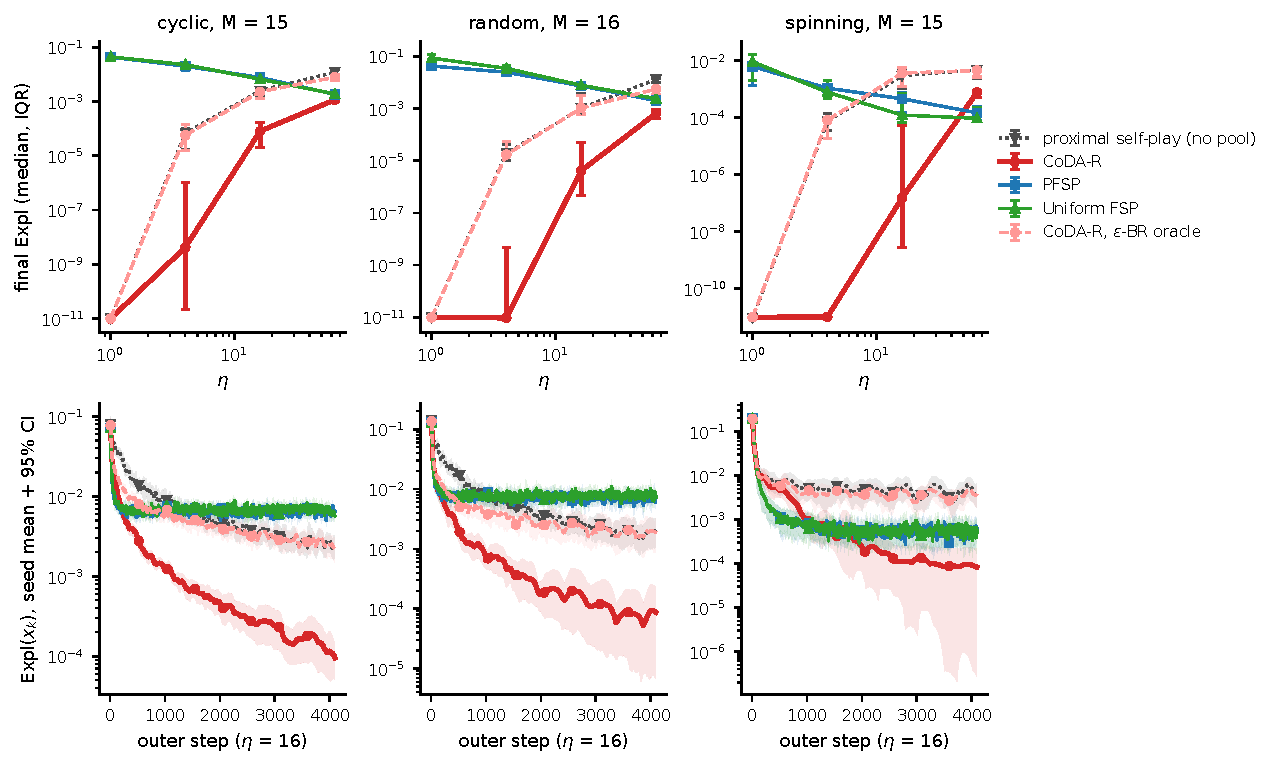
\includegraphics[width=0.92\linewidth]{figures/theory_oracle_rate.pdf}
\end{center}
\vspace{-6pt}
\caption{Effect of a best-response oracle on the exact algorithm (10 games per family). Top: final exploitability against $\eta$ (median and interquartile range). Bottom: exploitability over steps at $\eta=16$. Proximal self-play is \codar{} with an empty pool; PFSP and uniform FSP use the same pool as \codar{}.}
\label{fig:oracle-rate}
\end{figure}

\textbf{Oracle speed-up.} A best-response oracle speeds up \codar{} as Theorem~\ref{thm:oracle} predicts (Figure~\ref{fig:oracle-rate}). With the exact best response to the policy anchor added at every step, the inequality of the theorem holds at every step of all 240 \codar{} runs. For every $\eta\ge4$ and all three game families, \codar{} ends at a lower exploitability than the empty pool, for example $4\times10^{-6}$ against $10^{-3}$ on random $16\times16$ games at $\eta=16$; at $\eta=1$ both reach the numerical floor. PFSP and uniform weights with the same pool stall near $10^{-2}$ at small $\eta$, because they keep a fixed share on exploiters that tie the learner at the equilibrium. An oracle with error $0.01$ helps only while exploitability is above the scale of its error and ends close to the empty pool, as the theorem suggests. The one exception to the ordering is spinning-top games at $\eta=64$, where PFSP and uniform weights end lower ($1.5\times10^{-4}$ and $9.5\times10^{-5}$ against $7.6\times10^{-4}$).

\subsection{Matched-Budget Comparison}
\label{sec:exp-neural}

We compare \codar{} with seven baselines on Leduc poker~\citep{southey2005bayesbluff}, Goofspiel(4)~\citep{ross1971goofspiel}, and Liar's Dice with one die each~\citep{lisy2015oos} in OpenSpiel~\citep{lanctot2019openspiel}. The single-network baselines are PPO self-play; two regularized self-play methods, \rnad{} and MMD-PPO, which implement the proximal term as reward shaping and as a KL loss; and two pool methods, uniform fictitious self-play (FSP) and PFSP. The pool methods share the pool, the oracle, the loss estimator, and the policy update with \codar{} and differ only in the rule that maps loss estimates to weights, so \codar{} versus PFSP isolates the weight rule. The mixture baselines are PSRO with PPO best responses and Neural Fictitious Self-Play (NFSP)~\citep{heinrich2016nfsp}. We also run \codar{} without an oracle and, as upper-bound controls, \codar{}, PFSP, and PSRO with an exact best-response (BR) oracle that consumes no games. All PPO methods share the network and the PPO hyperparameters, and every method is tuned by the same two-stage protocol on held-out seeds (Appendix~\ref{app:impl}). Each run has a budget of $B=4\times10^6$ games, which counts every game a method consumes, including exploiter training and evaluation. We report exact full-tree exploitability, in chips for Leduc and in units of the $\pm1$ payoff for the other games, and summarize each run by its \emph{tail exploitability}, the mean over the last 20\% of the budget. Tables give the interquartile mean (IQM) with a bootstrap 95\% confidence interval (CI) over 10 seeds~\citep{agarwal2021precipice}, together with per-seed paired differences.

\begin{figure}[t]
\begin{center}
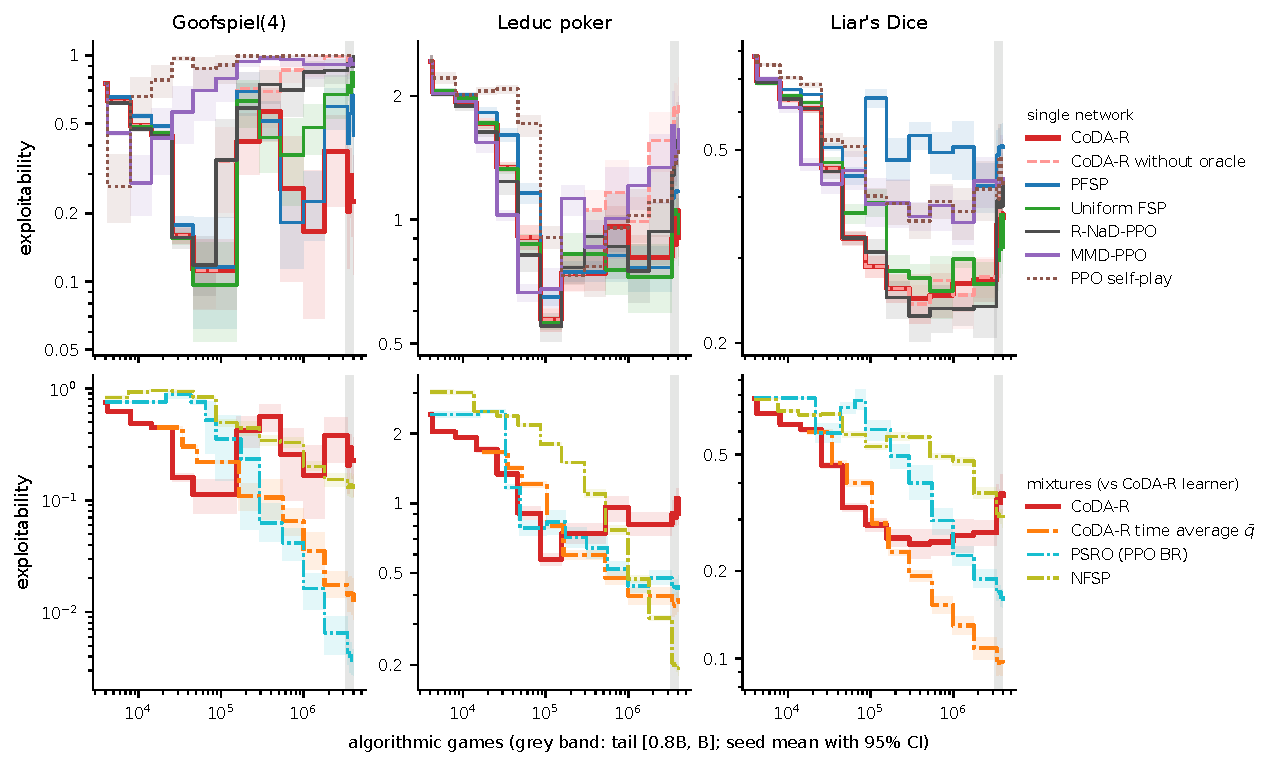
\includegraphics[width=0.95\linewidth]{figures/main_curves.pdf}
\end{center}
\vspace{-6pt}
\caption{Exact exploitability during training (seed mean and 95\% CI, 10 seeds). Top: single networks. Bottom: mixtures, with the \codar{} learner repeated for reference. The gray band marks the last 20\% of the budget.}
\label{fig:main}
\end{figure}

\begin{table}[t]
\caption{Tail exploitability at a matched budget (IQM [95\% CI] over 10 seeds; lower is better). Bold: best single network per game. The exact-BR rows are upper-bound controls. Further metrics are in Appendix Table~\ref{tab:main-full}.}
\label{tab:main}
\begin{center}
\scriptsize
\setlength{\tabcolsep}{3pt}
\begin{tabular}{llccc}
\toprule
Method & Deploy & Goofspiel(4) & Leduc poker & Liar's Dice \\
\midrule
PPO self-play & single & 0.999 [0.997, 1.000] & 1.287 [1.064, 1.705] & 0.445 [0.379, 0.501] \\
\rnad{} & single & 0.941 [0.858, 0.997] & 1.433 [1.345, 1.572] & 0.390 [0.360, 0.433] \\
MMD-PPO & single & 0.943 [0.863, 0.990] & 1.618 [1.416, 1.825] & 0.442 [0.368, 0.494] \\
Uniform FSP & single & 0.732 [0.662, 0.807] & 1.030 [0.928, 1.125] & \textbf{0.307} [0.286, 0.351] \\
PFSP & single & 0.517 [0.445, 0.590] & 1.150 [0.932, 1.297] & 0.479 [0.447, 0.502] \\
\codar{} without oracle & single & 0.973 [0.866, 0.997] & 1.699 [1.483, 1.931] & 0.379 [0.316, 0.434] \\
\codar{} & single & \textbf{0.256} [0.221, 0.295] & \textbf{0.919} [0.880, 0.975] & 0.355 [0.322, 0.378] \\
\midrule
NFSP & mixture & 0.116 [0.102, 0.164] & 0.196 [0.192, 0.200] & 0.308 [0.290, 0.329] \\
PSRO (PPO BR) & mixture & 0.0040 [0.0031, 0.0050] & 0.433 [0.394, 0.480] & 0.163 [0.156, 0.172] \\
\codar{} time average $\bar{\bq}$ & mixture & 0.0114 [0.0088, 0.0194] & 0.373 [0.324, 0.417] & 0.094 [0.084, 0.110] \\
\midrule
\codar{}, exact-BR oracle & single & 0.215 [0.138, 0.308] & 0.885 [0.797, 0.973] & 0.269 [0.241, 0.294] \\
PFSP, exact-BR oracle & single & 0.343 [0.301, 0.409] & 0.709 [0.625, 0.778] & 0.401 [0.375, 0.428] \\
PSRO, exact BR & mixture & $<10^{-15}$ & 0.108 [0.106, 0.115] & 0.172 [0.168, 0.175] \\
\bottomrule
\end{tabular}
\end{center}
\end{table}

\begin{table}[t]
\caption{Per-seed paired differences in tail exploitability (first minus second; IQM [95\% CI]), with the number of seeds out of 10 on which the first is better.}
\label{tab:paired}
\begin{center}
\scriptsize
\setlength{\tabcolsep}{2.5pt}
\begin{tabular}{lccc}
\toprule
Pair & Goofspiel(4) & Leduc poker & Liar's Dice \\
\midrule
\codar{} $-$ \rnad{} & $-0.659$ [$-0.747$, $-0.586$] (10) & $-0.503$ [$-0.662$, $-0.399$] (10) & $-0.051$ [$-0.097$, $-0.005$] (8) \\
\codar{} $-$ MMD-PPO & $-0.677$ [$-0.753$, $-0.554$] (10) & $-0.713$ [$-0.897$, $-0.519$] (10) & $-0.097$ [$-0.149$, $-0.034$] (9) \\
\codar{} $-$ PFSP & $-0.261$ [$-0.331$, $-0.163$] (10) & $-0.204$ [$-0.373$, $-0.017$] (7) & $-0.131$ [$-0.187$, $-0.065$] (10) \\
\codar{} $-$ Uniform FSP & $-0.500$ [$-0.580$, $-0.388$] (10) & $-0.139$ [$-0.218$, $+0.014$] (7) & $+0.045$ [$-0.033$, $+0.084$] (3) \\
\codar{} $-$ \codar{} without oracle & $-0.693$ [$-0.769$, $-0.574$] (10) & $-0.761$ [$-1.010$, $-0.588$] (10) & $-0.037$ [$-0.077$, $+0.013$] (7) \\
\codar{} $-$ PFSP, both exact-BR & $-0.089$ [$-0.224$, $-0.020$] (10) & $+0.200$ [$+0.071$, $+0.293$] (2) & $-0.122$ [$-0.165$, $-0.095$] (10) \\
$\bar{\bq}$ $-$ PSRO (PPO BR) & $+0.007$ [$+0.004$, $+0.016$] (0) & $-0.078$ [$-0.112$, $-0.007$] (8) & $-0.069$ [$-0.089$, $-0.046$] (10) \\
$\bar{\bq}$ $-$ NFSP & $-0.106$ [$-0.146$, $-0.091$] (10) & $+0.178$ [$+0.128$, $+0.218$] (0) & $-0.208$ [$-0.220$, $-0.199$] (10) \\
\bottomrule
\end{tabular}
\end{center}
\end{table}

Among single networks, \codar{} has the lowest tail exploitability on Goofspiel(4) and Leduc poker (Tables~\ref{tab:main} and~\ref{tab:paired}). It beats \rnad{}, MMD-PPO, and \codar{} without an oracle on all 10 seeds in both games, and its tail exploitability is 73\% and 36\% below that of \rnad{}. Against PFSP, which differs only in the weight rule, it is better on 10/10 seeds on Goofspiel(4) and 7/10 on Leduc. On Liar's Dice it beats \rnad{}, MMD-PPO, and PFSP and is second to uniform FSP, with a paired difference whose CI includes zero.

Methods without a pool degrade after an early optimum, and \codar{} largely holds its level (Figure~\ref{fig:main}). On Goofspiel(4) and Leduc, the methods without a pool reach their lowest exploitability within the first 10\% of the budget and end 0.7--1.1 above it, while \codar{} ends 0.25--0.36 above its lowest point (Appendix Table~\ref{tab:degradation}). Without the oracle, \codar{} loses most of its gain on these two games, so the gain comes from the exploiters that enter the pool. The remaining spikes of \codar{}, with a worst tail exploitability of 0.80 on Goofspiel(4), are due to loss estimates that lag behind abrupt jumps of the true loss rates: 14 of the 17 vulnerabilities detected there had weight below 0.01 when they opened, and exact member losses lower the tail exploitability in the ablation of \S\ref{sec:exp-abl}.

A stronger oracle helps \codar{} on Liar's Dice ($0.355\to0.269$) and changes little on the other two games. With exact best responses, PFSP is ahead on Leduc (0.709 against 0.885): an exploiter's lead there is a small fraction of the 26-chip payoff range, so the weight $c\mu/2$ stays small, whereas PFSP gives the pool a fixed half of the training weight.

The time average $\bar{\bq}$ of the same \codar{} run is competitive with the dedicated mixture methods. It only requires storing one snapshot per outer step, and it beats PSRO with the same PPO best responses on Leduc (8/10 seeds) and Liar's Dice (10/10) and comes close on Goofspiel(4) (0.011 against 0.004); NFSP is better on Leduc. The single learner stays above these mixtures on all three games.

Exploiter leads give calibrated lower bounds on exploitability. Each oracle admission yields the bound $[\ell(\hat\bx;\hat\by)-\tfrac12]^+$ of \S\ref{sec:oracle-rate}, estimated from evaluation games. Over 3950 admissions in the main runs, the one-sided 95\% confidence bound exceeded the true exploitability 3 times, and it was positive, i.e., informative, 2487 times.

\subsection{Scaling to Large Games}
\label{sec:exp-scale}

We train six methods on 3$\times$3 abrupt Dark Hex and abrupt Phantom Tic-Tac-Toe, two imperfect-information games with about $2.7\times10^{10}$ nodes and $2.7\times10^{7}$ and $2.3\times10^{7}$ information sets, with the same budget and 5 seeds. The methods reuse the configurations selected on Goofspiel(4) without further tuning. Exploitability is computed exactly over the full tree with exp-a-spiel~\citep{rudolph2025reevaluating}, and the tail exploitability averages the checkpoints at $0.8B$, $0.9B$, and $B$.

\begin{table}[t]
\caption{Large games: tail exploitability (IQM [95\% CI], 5 seeds) and the per-seed paired difference \codar{} $-$ method, with the number of seeds out of 5 on which \codar{} is better.}
\label{tab:scale}
\begin{center}
\scriptsize
\setlength{\tabcolsep}{3pt}
\begin{tabular}{llcccc}
\toprule
 & & \multicolumn{2}{c}{3$\times$3 abrupt Dark Hex} & \multicolumn{2}{c}{Abrupt Phantom TTT} \\
Method & Deploy & tail exploitability & \codar{} $-$ method & tail exploitability & \codar{} $-$ method \\
\midrule
PPO self-play & single & 0.971 [0.837, 0.993] & $-0.531$ [$-0.592$, $-0.376$] (5) & 0.961 [0.893, 0.985] & $-0.439$ [$-0.464$, $-0.409$] (5) \\
\rnad{} & single & 0.529 [0.438, 0.598] & $-0.108$ [$-0.174$, $+0.023$] (4) & \textbf{0.509} [0.490, 0.568] & $-0.009$ [$-0.062$, $+0.041$] (2) \\
MMD-PPO & single & 0.542 [0.524, 0.583] & $-0.109$ [$-0.182$, $-0.054$] (5) & 0.641 [0.604, 0.751] & $-0.126$ [$-0.279$, $-0.062$] (5) \\
PFSP & single & 0.743 [0.710, 0.794] & $-0.333$ [$-0.361$, $-0.237$] (5) & 0.832 [0.773, 0.893] & $-0.316$ [$-0.402$, $-0.246$] (5) \\
\codar{} & single & \textbf{0.432} [0.395, 0.476] & --- & 0.512 [0.467, 0.551] & --- \\
\midrule
PSRO (PPO BR) & mixture & 0.355 [0.290, 0.386] & $+0.092$ [$+0.010$, $+0.159$] (0) & 0.525 [0.495, 0.529] & $-0.014$ [$-0.061$, $+0.055$] (4) \\
\bottomrule
\end{tabular}
\end{center}
\end{table}

\codar{} has the lowest tail exploitability among single networks on Dark Hex and ties \rnad{} on Phantom Tic-Tac-Toe, where the two differ by 0.009 with a CI that includes zero (Table~\ref{tab:scale}). It matches the PSRO mixture on Phantom Tic-Tac-Toe and is 0.09 behind it on Dark Hex. PFSP, with the same pool and oracle, is much worse on both games (0.74 and 0.83), and self-play is almost fully exploitable. In a sampled round-robin among the final policies, \codar{} has the highest average score on Dark Hex (0.510) and is within 0.001 of the highest on Phantom Tic-Tac-Toe. Playing every checkpoint against its own earlier checkpoints shows that only self-play loses to its past selves, on 25--29\% of its checkpoints; for \codar{}, the worst lead of an earlier checkpoint, averaged over checkpoints, is 0.009 on Dark Hex and negative on Phantom Tic-Tac-Toe (Appendix Figure~\ref{fig:scale-history}).

\subsection{What the Pool Buys}
\label{sec:exp-mech}

The main comparison mixes several effects. Four controlled experiments on Leduc and Goofspiel(4), with 6 seeds each and the configurations of the main comparison, separate them (settings and full tables in Appendix~\ref{app:mech}).

\begin{figure}[t]
\begin{center}
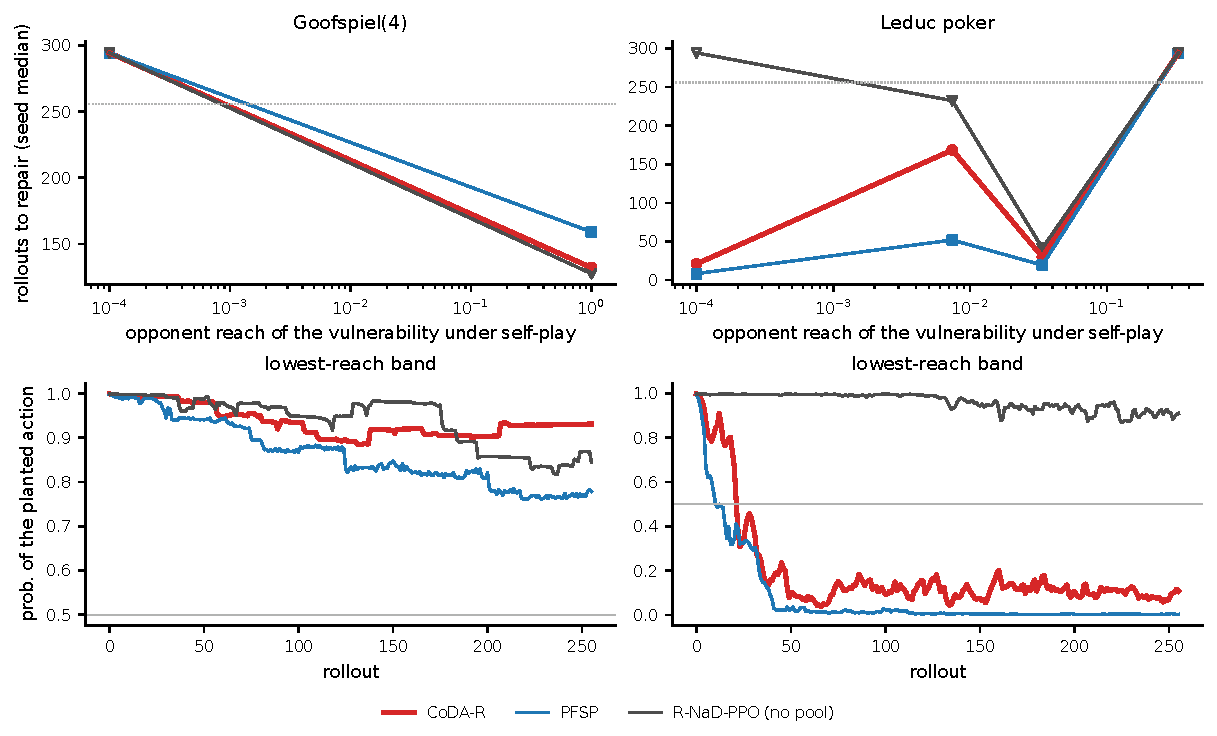
\includegraphics[width=0.78\linewidth]{figures/hidden_hole.pdf}
\end{center}
\vspace{-6pt}
\caption{Hidden vulnerabilities (6 seeds). Top: median number of rollouts to repair against the probability with which self-play opponents reach the planted vulnerability; points above the dotted line were not repaired. Bottom: probability of the planted action in the band with the lowest reach.}
\label{fig:mech}
\end{figure}

\begin{figure}[t]
\begin{center}
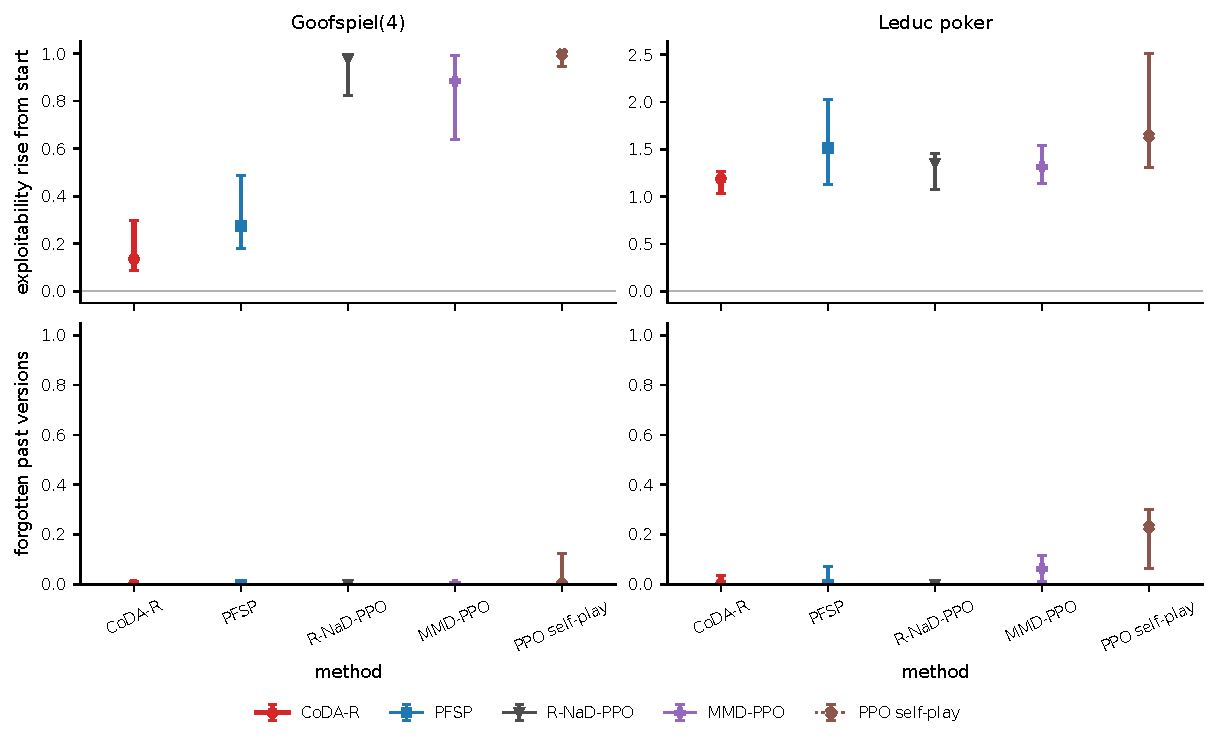
\includegraphics[width=0.78\linewidth]{figures/forgetting.pdf}
\end{center}
\vspace{-6pt}
\caption{Retention from a near-Nash start (IQM and 95\% CI, 6 seeds). Top: rise of exploitability over the starting network. Bottom: fraction of archived earlier versions that later beat the learner again.}
\label{fig:retention}
\end{figure}

\textbf{Hidden vulnerabilities.} A pool repairs vulnerabilities that self-play almost never reaches. We distill the average strategy of counterfactual regret minimization (CFR+)~\citep{tammelin2014cfrplus} into a network and plant vulnerabilities at information sets that the learner itself reaches often but that self-play opponents reach with a controlled probability, from $[0.3,1)$ down to below $10^{-3}$. The pool holds only the exact best response to the damaged network, and \rnad{} trains without it. On Leduc (Figure~\ref{fig:mech}), the repair time of \rnad{} grows as the opponent reach falls, and in the lowest band, with reach about $2\times10^{-6}$, it repairs the vulnerability on none of 6 seeds within 256 rollouts. With the attacker in the pool, \codar{} repairs it on all 6 (median 21 rollouts), and so does PFSP (median 8.5). PFSP is faster because it gives the attacker a fixed coefficient of about 0.17, against 0.03--0.06 under \codar{}, whose weight follows the attacker's small lead of about 0.02. The fixed coefficient costs exploitability, which in the lowest band ends at 1.61 for PFSP against 1.30 for \codar{} and 1.81 for \rnad{}. On Goofspiel(4) no method repairs the lowest band, because the learner counters the deterministic attacker on other branches, and the attacker stops winning while the vulnerability stays open.

\textbf{Retention.} A pool keeps a near-Nash network near Nash. Starting from the same distilled network without planted vulnerabilities (exploitability $3.8\times10^{-4}$ on Goofspiel(4) and $0.0088$ on Leduc), we train each method for $10^6$ more games. On Goofspiel(4) (Figure~\ref{fig:retention}), the methods without a pool lose the equilibrium almost entirely: exploitability rises by 0.98 for \rnad{}, 0.88 for MMD-PPO, and 1.00 for self-play. For \codar{} it rises by 0.14 [0.09, 0.30], less than for each method without a pool on all 6 seeds, and for PFSP by 0.28, so retention is a property of the pool. On Leduc every method drifts back to roughly its level in the main comparison, and \codar{} rises least (1.19 against 1.32--1.64; significant only against self-play). The drift is concentrated where self-play does not go. At information sets that self-play opponents reach with probability below $10^{-3}$, the per-visit loss relative to the start on Leduc is 0.0030 for \codar{} and 0.0040 for PFSP, against 0.0093--0.0157 for the methods without a pool, while the bands with higher reach are similar (Appendix Figure~\ref{fig:drift}). Hidden vulnerabilities and drift thus share one mechanism: self-play produces no gradient where it does not go, parameter sharing lets those parts of the policy drift, and pool members that do go there supply the missing signal. Cycling back to beaten versions is a separate effect that the proximal term alone already prevents: against an archive of its own earlier versions, only self-play (23\% of versions on Leduc) and MMD-PPO (6\%) lose to versions they had beaten. Halving or doubling $c$ leaves these results unchanged.

\textbf{Sleeper members.} \codar{} returns weight to a member as soon as it wins again and spends little training on members that no longer win. Weights that accumulate history, such as Hedge, leave a member that has been suppressed for $T$ rounds ``asleep'': it has to win for about $T$ more rounds to regain its weight. We place the exact best response to an \rnad{} base network in the pool together with three random-network decoys, let each rule suppress it for $T\in\{24,48,96,192\}$ rollouts, and then reset the learner to the base, which reopens the vulnerability. With \codar{}, the time to repair it again does not depend on $T$ (about 1 rollout on Goofspiel(4) and 3--6 on Leduc). Hedge needs 31.5 and 37.7 rollouts at $T=192$ (Appendix Figure~\ref{fig:sleeper}), and \rnad{} without a pool does not repair Leduc again within 96 rollouts at $T=192$. Members that do not beat the learner ($\ell\le0.51$) hold 0.6--1.5\% of the training weight under \codar{} on Goofspiel(4) and 11--13\% on Leduc, against 44--50\% for PFSP and Hedge and 28--35\% for fixed mixing. On Leduc the rules with a fixed share end at a lower tail exploitability in this setting (0.57--0.65 for PFSP and 0.48--0.59 for fixed mixing, against 0.72--0.81). The moving anchor behaves like \codar{} here, since its failure requires a tied pool.

\textbf{Open pools.} With a pool of external agents and no oracle, \codar{} keeps its training on the members that still beat the learner. With 4 to 64 external members (early CFR+ iterates, small legacy networks, scripted bots, the uniform policy, random networks, and duplicates), members that the learner already beats hold 0.3--1.1\% of the training weight under \codar{} on Goofspiel(4) and 4--6\% on Leduc, against 42--46\% under PFSP and 9--19\% under uniform FSP, independently of the pool size (Appendix Figure~\ref{fig:open-pool}). Exploitability under every rule then depends on what the pool members know, and this pool does not lower it reliably without an oracle.

\subsection{Ablations}
\label{sec:exp-abl}

Appendix Figure~\ref{fig:ablations} changes one design element of \codar{} at a time ($10^6$ games, 6 seeds, paired against the base configuration). The oracle matters most: removing it raises the tail exploitability by 0.76 on Goofspiel(4) and 0.42 on Leduc. Freezing the pool weights for a whole outer step, which breaks the implicit pairing of \S\ref{sec:primal}, costs 0.38 and 0.15, and a pool capacity of 4 costs 0.32 and 0.24. Exact member losses ($\xi_k=0$) help on Goofspiel(4) ($-0.09$, 6/6 seeds), which identifies estimation lag as the main remaining error there, and doubling the oracle's share of the budget to 24\% helps on Leduc ($-0.20$, 5/6 seeds). The moving dual anchor, the sampling distribution, the refresh rate of the self-play opponent, and the KL form of the proximal term change the tail exploitability within the CIs at this budget; the failure of the moving anchor appears in the exact setting of \S\ref{sec:exp-theory}.

% ----------------------------------------------------------------------
\section{Related Work}
\label{sec:related}
% ----------------------------------------------------------------------

Population methods keep a pool of opponents and place the equilibrium in a mixture. Double Oracle and PSRO~\citep{mcmahan2003doubleoracle,lanctot2017psro,muller2020generalized,mcaleer2020pipeline} solve a meta-game over the pool externally~\citep{wellman2006egta}, PFSP and league training~\citep{vinyals2019alphastar} allocate sampling proportions by win rate, and NFSP~\citep{heinrich2015fsp,heinrich2016nfsp} learns the historical average strategy with a separate network. What they deploy is a mixture of checkpoints or the average network. \codar{} uses the same kind of pool and oracle and keeps the guarantee on the network being trained.

Regularized self-play gives a guarantee for a single network, without a pool. R-NaD and MMD~\citep{perolat2021rnad,perolat2022stratego,sokota2023mmd} use an anchor in payoff or policy space that moves periodically or is annealed, and optimistic and extragradient methods~\citep{daskalakis2018optimism,mertikopoulos2019omd,nemirovski2004prox,cen2021extragradient} stabilize similarly with an extrapolation term; both are explicit approximations~\citep{mokhtari2020ppa} of the proximal point method~\citep{rockafellar1976ppa}. They train only along the self-play trajectory, which is why OpenAI Five and AlphaStar also keep historical opponents~\citep{openai2019dota,vinyals2019alphastar,czarnecki2020spinning}. The policy update of \codar{} is the proximal point step itself, and with an empty pool \codar{} reduces to it.

Multiplicative weights accumulate history, which the stateless projection of \codar{} avoids. The meta-solvers of the PSRO family, namely Hedge, projected replicator dynamics, and the multiplicative weights update (MWU), and the opponent sampler of OpenAI Five mostly use multiplicative weights~\citep{lanctot2017psro,mcaleer2022anytime,dinh2022odo,openai2019dota,freund1999hedge}. After a member has been suppressed for $T$ rounds, it has to win for roughly another $T$ rounds to regain its weight even if it counters the learner again. This is the sleeper problem that Fixed Share-type algorithms address in online learning~\citep{herbster1998tracking}. Conversely, tied members keep positive weight indefinitely. Methods that deploy the time average are unaffected, but the last iterate of multiplicative weights does not converge in zero-sum games~\citep{bailey2018mwu}, and tied members that keep their weight can pin the learner at a non-Nash point (Proposition~\ref{prop:rps}). Appendix Table~\ref{tab:related} compares the methods.

% ----------------------------------------------------------------------
\section{Conclusion}
% ----------------------------------------------------------------------

\codar{} trains a single network against itself and an open pool of opponents. Fixing the dual anchor at pure self-play and placing the moving anchor in the policy update makes policy movement and pool weight draw on one budget, the distance to equilibrium. For the exact algorithm, this gives last-iterate convergence of the trained policy for any sequence of pools, explicit rates, and a quantified gain from a best-response oracle. With PPO, at a matched budget and against baselines tuned by the same protocol, the \codar{} learner has the lowest tail exploitability among single networks on Goofspiel(4), Leduc poker, and 3$\times$3 abrupt Dark Hex, ties \rnad{} on abrupt Phantom Tic-Tac-Toe, and is second to uniform FSP on Liar's Dice. Controlled experiments show that the pool repairs vulnerabilities that self-play almost never reaches and keeps a near-Nash network in place, and that the weight rule returns weight to a reopened vulnerability at once and spends little training on members that no longer win. Because the weight follows an opponent's lead, small leads are repaired more slowly than under the fixed share of PFSP. Detecting small leads faster, a KL version of the Euclidean theory, and a last-iterate rate across pool changes are the main open directions.

\subsubsection*{Reproducibility Statement}
\S\ref{sec:prelim}--\ref{sec:alg} give all definitions of the algorithm, and \S\ref{sec:theory} together with Appendix~\ref{app:proofs} gives all proofs. \S\ref{sec:impl} and Appendix~\ref{app:impl} give the implementation, the evaluation protocol, the tuning grids, and every selected configuration. The source code includes the finite-dimensional solver and checks, the PPO implementation, all baselines, the experiment entry points with all configurations and seeds, and the scripts that generate every figure and table from the raw outputs; it is open source on the author's GitHub at \url{https://github.com/GICF-E/CoDA-R}.

\subsubsection*{AI Use Statement}
In this work, we used generative AI tools to assist with drafting and polishing the text of the paper, writing and refactoring experiment code, formatting references, and aggregating experiment logs to generate figures and tables. Regarding research content, AI tools were used to refine the formulation of research hypotheses, to assist with derivations and the checking of proof steps, and to assist with interpreting experimental results. The core algorithm, theorem statements, and research design were proposed by the authors. We did not use generative AI to generate synthetic data or to fabricate experimental results. All AI-assisted code was tested and type-checked by the authors, and all AI-assisted proofs, interpretations, and text were manually reviewed item by item by the authors. The authors take responsibility for the entire content of this paper.

\bibliography{references}
\bibliographystyle{plainnat}

% ----------------------------------------------------------------------
\appendix
\section{Proofs}
\label{app:proofs}
% ----------------------------------------------------------------------

The main text proves Lemmas~\ref{lem:A} and~\ref{lem:B} and Theorem~\ref{thm:energy}. This appendix proves the remaining results, in the order in which they appear, using only the tools listed in \S\ref{sec:prelim}. Throughout, $\bx:=\bx_{k+1}$, $\bw:=\bw(\bx)$, $\bv:=\bv_{k+1}$, and $\dx_k=\bx_{k+1}-\bx_k$.

\subsection{Lemma~\ref{lem:dual}: Properties of the Weight Rule}
\label{app:dual}

Let $\bz:=\esp+c\aug(\bx)$, so that $\bw=\Proj_\simplex(\bz)$, and write $z_{\mathrm{sp}}=1+\tfrac c2$ for the self-play coordinate of $\bz$.

(a) By the projection inequality, $\esp=\Proj_\simplex(\bz)$ if and only if $(\bz-\esp)^\top(\bu-\esp)\le0$ for all $\bu\in\simplex$. Since $\bz-\esp=c\aug$, the condition becomes $\aug^\top \bu\le\aug^\top \esp=\tfrac12$ for all $\bu$. A linear function attains its maximum over the simplex at a vertex, so this means $\max_j\tilde\ell_j\le\tfrac12$. The self-play coordinate is exactly $\tfrac12$, so this is equivalent to $\max_{i\in P}\ell_i\le\tfrac12$.

(b) Move a little weight from member $i$ to self-play by taking $\bu=\bw+\theta(\esp-\be_i)$ with $0<\theta\le w_i$, which remains in $\simplex$. The projection inequality gives
\[
(\bz-\bw)^\top(\bu-\bw)=\theta\big[(z_{\mathrm{sp}}-\wsp)-(z_i-w_i)\big]\le0
\iff c\,\ell_i-w_i\ \ge\ z_{\mathrm{sp}}-\wsp=1+\tfrac c2-\wsp ,
\]
i.e., $c(\ell_i-\tfrac12)\ge1-\wsp+w_i\ge w_i>0$.

(c) The points of $\simplex_2$ are $(\theta,1-\theta)$ with $\theta\in[0,1]$, and their squared distance to $\bz=(\tfrac c2+c\mu,\ 1+\tfrac c2)$,
\[
(\tfrac c2+c\mu-\theta)^2+(\tfrac c2+\theta)^2 ,
\]
is a convex quadratic function of $\theta$ with unconstrained minimizer $\theta=\tfrac{c\mu}2$; the minimizer over $[0,1]$ is obtained by clipping it to the interval.\hfill$\blacksquare$

\subsection{Unique Solution of the Policy Update}
\label{app:unique}

\begin{proposition}[Unique solution at each step]
\label{prop:unique}
For any policy anchor $\bx_k$ and any pool, \eqref{eq:P} has one and only one solution.
\end{proposition}
Uniqueness comes from three facts: the self-play term is skew-symmetric, the pool term is monotone by the monotonicity of the projection, and the proximal term is $\eta$-strongly monotone. Existence follows from the Hartman--Stampacchia theorem. Denote the operator of the first two terms by $G_k(\bx):=S\bx+A\bw(\bx)_P$.

\textit{$G_k$ is monotone.} For the self-play term, $(\bx-\bx')^\top S(\bx-\bx')=0$, so $\langle S(\bx-\bx'),\bx-\bx'\rangle=0$. For the pool term, let $\bz=\esp+c\aug(\bx)$ and $\bz'=\esp+c\aug(\bx')$. The self-play coordinates coincide and the pool coordinates differ by $c(\ell_i(\bx)-\ell_i(\bx'))=c\,(S\by_i)^\top(\bx-\bx')$, i.e., $(\bz-\bz')_P=c\,A^\top(\bx-\bx')$. By \eqref{eq:monotone},
\[
0\le(\bz-\bz')^\top\big(\bw(\bx)-\bw(\bx')\big)=(\bz-\bz')_P^\top\big(\bw(\bx)-\bw(\bx')\big)_P=c\,(\bx-\bx')^\top A\big(\bw(\bx)-\bw(\bx')\big)_P ,
\]
i.e., $\langle A\bw(\bx)_P-A\bw(\bx')_P,\bx-\bx'\rangle\ge0$. After adding $\eta(\bx-\bx_k)$, the whole operator satisfies $\langle\cdot,\bx-\bx'\rangle\ge\eta\|\bx-\bx'\|^2$, i.e., it is $\eta$-strongly monotone. This uses that the self-play coefficient does not depend on $\bx$; a coefficient such as $\wsp(\bx)$ would turn the self-play term into $\wsp(\bx)S\bx$, which is no longer a skew-symmetric quadratic form.

\textit{Uniqueness.} Suppose $\bx$ and $\bx'$ both solve \eqref{eq:P}. Take the test point $\bx'$ in the inequality for $\bx$ and the test point $\bx$ in the inequality for $\bx'$:
\[
\langle G_k(\bx)+\eta(\bx-\bx_k),\,\bx'-\bx\rangle\ge0,\qquad\langle G_k(\bx')+\eta(\bx'-\bx_k),\,\bx-\bx'\rangle\ge0 .
\]
Adding them gives $\eta\|\bx-\bx'\|^2\le-\langle G_k(\bx)-G_k(\bx'),\bx-\bx'\rangle\le0$, so $\bx=\bx'$.

\textit{Existence.} $\aug$ is affine and $\bw(\bx)$ is continuous by the nonexpansiveness in \eqref{eq:monotone}, so $G_k$ is continuous, and $X$ is compact and convex. A variational inequality with a continuous operator on a compact convex set has a solution, which is the Hartman--Stampacchia theorem~\citep{hartman1966,facchinei2003vi}.\hfill$\blacksquare$

\subsection{Theorem~\ref{thm:cert}: Two Certificates}
\label{app:cert}

(i) Take $\by_e\in\arg\max_\by\ell(\bx;\by)$. Then $\bx^\top S\by_e=\Expl(\bx)$, and skew-symmetry gives $\by_e^\top S\bx=-\Expl(\bx)$. Take $\bx'=\by_e$ in \eqref{eq:P}, let $\bg:=\by_e-\bx$, and separate the three terms:
\[
\underbrace{(S\bx)^\top \bg}_{\text{self-play}}+\underbrace{(A\bw_P)^\top \bg}_{\text{pool}}+\underbrace{\eta\,\dx_k^\top \bg}_{\text{proximal}}\ \ge\ 0 .
\]
The self-play term is $(S\bx)^\top \bg=\by_e^\top S\bx-\bx^\top S\bx=-\Expl(\bx)$. For the pool term, using $(S\by_i)^\top \bz=\ell_i(\bz)-\tfrac12$,
\[
(A\bw_P)^\top \bg=\sum_iw_i\big(\ell_i(\by_e)-\ell_i(\bx)\big)=\sum_iw_i\big(\ell_i(\by_e)-\tfrac12\big)-b\ \le\ \tfrac12a-b ,
\]
where the last step uses that loss rates are at most 1. For the proximal term, Cauchy--Schwarz and the diameter give $\eta\,\dx_k^\top \bg\le\eta D\|\dx_k\|$. Combining the three terms gives $-\Expl(\bx)+\tfrac12a-b+\eta D\|\dx_k\|\ge0$, and rearranging yields the first inequality; the second uses $b\ge0$.

(ii) Apply the projection inequality to $\bw=\Proj_\simplex(\esp+c\aug)$ with $\bu=\be_j$, where $j$ is any pool member:
\[
\big(\esp+c\aug-\bw\big)^\top(\be_j-\bw)\le0\iff c\,\aug^\top(\be_j-\bw)\le(\bw-\esp)^\top(\be_j-\bw)\le\sqrt2\,\|\bw-\esp\| .
\]
By \eqref{eq:identities}, the left-hand side equals $c(\ell_j-\tfrac12-b)$, so $\ell_j-\tfrac12\le\frac{\sqrt2}c\|\bw-\esp\|+b$. By Lemma~\ref{lem:B} and Cauchy--Schwarz, $b\le\eta\,\dx_k^\top(\xs-\bx)\le\eta D\|\dx_k\|$. Taking $j$ to be the member with the largest loss rate, the right-hand side is nonnegative, so taking the positive part does not affect the bound.\hfill$\blacksquare$

\subsection{Theorem~\ref{thm:conv}: Convergence of the Learner}
\label{app:conv}

Corollary~\ref{cor:sum} gives $a\to0$ and $\|\dx_k\|\to0$, and substituting into Theorem~\ref{thm:cert}(i) gives $\Expl(\bx_{k+1})\le\tfrac12a+\eta D\|\dx_k\|\to0$. Since $X$ is compact and $\Expl$ is continuous, the limit $\bar \bx$ of any convergent subsequence is a Nash strategy. Theorem~\ref{thm:energy} holds with $\xs=\bar \bx$, so $\|\bx_k-\bar \bx\|$ is nonincreasing, and since it tends to zero along the subsequence, it tends to zero along the whole sequence.\hfill$\blacksquare$

\subsection{Theorem~\ref{thm:rate}: Rates}
\label{app:rate}

\textit{Proof of (i).} Let $\alpha_k=\|\bw(\bx_{k+1})-\esp\|$ and $\beta_k=\|\dx_k\|$. By Theorem~\ref{thm:cert}(i) and $a\le\alpha_k$, $\Expl(\bx_{k+1})\le\tfrac12\alpha_k+\eta D\beta_k$. The minimum is at most the average; applying Cauchy--Schwarz to each of the two sums ($\sum_{k<K}\alpha_k\le\sqrt K\sqrt{\sum\alpha_k^2}$) and substituting Corollary~\ref{cor:sum},
\begin{align*}
\min_{k<K}\Expl(\bx_{k+1})\ &\le\ \frac1K\sum_{k<K}\Big(\tfrac12\alpha_k+\eta D\beta_k\Big)\\
&\le\ \frac{1}{\sqrt K}\Big(\tfrac12\sqrt{\tfrac{c\eta}{2}}+\eta D\Big)\|\bx_0-\xs\|\ \le\ \frac{\sqrt{c\eta}/2+2\eta}{\sqrt K},
\end{align*}
where the last step uses $\|\bx_0-\xs\|\le\sqrt2$ and $D=\sqrt2$.

\textit{The step length is nonincreasing while the pool is fixed.} With a fixed pool, two consecutive steps share the same operator $G(\bx):=S\bx+A\bw(\bx)_P$, which is monotone (Appendix~\ref{app:unique}). Take the test point $\bx_{k+2}$ in \eqref{eq:P} at step $k$ and $\bx_{k+1}$ at step $k+1$:
\[
\langle G(\bx_{k+1})+\eta\dx_k,\ \bx_{k+2}-\bx_{k+1}\rangle\ge0,\qquad\langle G(\bx_{k+2})+\eta\dx_{k+1},\ \bx_{k+1}-\bx_{k+2}\rangle\ge0 .
\]
Adding them, the $G$ part is $\le0$ by monotonicity, leaving $\eta\langle\dx_k-\dx_{k+1},\dx_{k+1}\rangle\ge0$, i.e., $\|\dx_{k+1}\|^2\le\dx_k^\top\dx_{k+1}\le\|\dx_k\|\|\dx_{k+1}\|$, so $\|\dx_{k+1}\|\le\|\dx_k\|$.

\textit{Proof of (ii).} With the pool unchanged over steps $K-n,\dots,K-1$, $\|\dx_k\|$ is nonincreasing there. Summing the energy inequality \eqref{eq:energy} from $\bx_{K-n}$ gives $n\|\dx_{K-1}\|^2\le\sum_{k=K-n}^{K-1}\|\dx_k\|^2\le\|\bx_{K-n}-\xs\|^2\le2$, i.e., $\beta:=\|\dx_{K-1}\|\le\sqrt{2/n}$. At $\bx=\bx_K$, Lemma~\ref{lem:B} and Cauchy--Schwarz give $b(\bx)\le\eta D\beta$, and Lemma~\ref{lem:A} with $a^2\le\|\bw-\esp\|^2$ gives $a(\bx)\le\sqrt{c\,b(\bx)}\le\sqrt{c\eta D\beta}$. Substituting into Theorem~\ref{thm:cert}(i),
\[
\Expl(\bx_K)\ \le\ \tfrac12\sqrt{c\eta D\beta}+\eta D\beta\ \le\ \sqrt{c\eta/2}\;n^{-1/4}+2\eta\,n^{-1/2},
\]
using $D=\sqrt2$.\hfill$\blacksquare$

\subsection{Proposition~\ref{prop:mix}: Mixtures}
\label{app:mix}

\textit{Proof of (i).} $\bq_{k+1}=\bv_{k+1}/t_k\in X$, because $\bv$ is a nonnegative combination of points in $X$ with total mass $t_k\ge1$. For any $\by\in X$, take $\bx'=\by$ in \eqref{eq:P}:
\[
\by^\top S\bv-\underbrace{\bx^\top S\bv}_{=b}+\eta\,\dx_k^\top(\by-\bx)\ge0
\ \Longrightarrow\
-\by^\top S\bv\ \le\ -b+\eta\,\dx_k^\top(\by-\bx)\ \le\ \eta D\|\dx_k\| .
\]
By skew-symmetry, the left-hand side equals $\bv^\top S\by=t_k\,\bq_{k+1}^\top S\by$, and maximizing over $\by$ gives $t_k\Expl(\bq_{k+1})\le\eta D\|\dx_k\|$.

\textit{Proof of (ii).} The intermediate step above, $-\by^\top S\bv_{k+1}\le\eta\,\dx_k^\top(\by-\bx_{k+1})$, holds at every step. By the polarization identity with reference point $\by$,
\[
2\,\dx_k^\top(\by-\bx_{k+1})=\|\bx_k-\by\|^2-\|\bx_{k+1}-\by\|^2-\|\dx_k\|^2\ \le\ \|\bx_k-\by\|^2-\|\bx_{k+1}-\by\|^2 ,
\]
and telescoping over $k<K$,
\[
T_K\,\bar{\bq}_K^\top S\by=-\by^\top S\sum_{k<K}\bv_{k+1}\ \le\ \tfrac\eta2\big(\|\bx_0-\by\|^2-\|\bx_K-\by\|^2\big)\ \le\ \tfrac\eta2\|\bx_0-\by\|^2\ \le\ \eta .
\]
Divide both sides by $T_K$ and maximize over $\by$; $T_K\ge K$ because every $t_k=1+a(\bx_{k+1})\ge1$.\hfill$\blacksquare$

\subsection{Theorem~\ref{thm:inexact}: Inexact Steps}
\label{app:inexact}

Let $\hat b:=\sum_iw_{k+1,i}(\hat\ell_{k,i}-\tfrac12)$ denote the pool pressure computed from the estimated loss rates, while $a$ and $b$ are defined with the actual weights and the true loss rates.

\textit{Energy inequality.} Lemma~\ref{lem:A} holds for the vector that is actually projected, with the same proof and $\aug$ replaced by $\hat{\bell}$, which gives $\|\bw_{k+1}-\esp\|^2\le c\hat b$. Switching back to the true loss rates,
\[
\hat b-b=\sum_iw_{k+1,i}\big(\hat\ell_{k,i}-\ell_i(\hat \bx_{k+1})\big)\le\sum_iw_{k+1,i}\,\xi_k=a\,\xi_k ,
\]
since only the pool coordinates carry error; the self-play coordinate is always $\tfrac12$. For Lemma~\ref{lem:B}, taking $\bx'=\xs$ in the relaxed \eqref{eq:P}, we again have ${\xs}^\top S\hat \bv\le0$, which gives $\eta\,\dx_k^\top(\xs-\hat \bx)\ge b-\delta_k$. Chaining these,
\[
\eta\,\dx_k^\top(\xs-\hat \bx)\ \ge\ b-\delta_k\ \ge\ \hat b-a\,\xi_k-\delta_k\ \ge\ \tfrac1c\|\bw_{k+1}-\esp\|^2-a\,\xi_k-\delta_k ,
\]
and substituting into the polarization identity gives the energy inequality.

\textit{Certificates and mixtures.} Repeat the proofs of Theorem~\ref{thm:cert} and Proposition~\ref{prop:mix} with two substitutions. The right-hand side of \eqref{eq:P} changes from $0$ to $-\delta_k$, which adds $\delta_k$ to every bound. Wherever $-b\le0$ was used, we now have $\hat b\ge0$ and hence $-b\le-\hat b+a\,\xi_k\le a\,\xi_k$, which adds $a\,\xi_k$ to the certificate of the learner and to each of the two mixture bounds. For the in-pool certificate, the projection inequality applied to $\esp+c\hat{\bell}$ gives $\hat\ell_j-\tfrac12\le\frac{\sqrt2}c\|\bw-\esp\|+\hat b$; switching back to the true loss rates uses $\ell_j\le\hat\ell_j+\xi_k$ and $\hat b\le b+a\,\xi_k\le b+\xi_k$, for a total of $2\xi_k$, and finally $b\le\eta D\|\dx_k\|+\delta_k$.

\textit{Summable errors.} If $\sum_k(\delta_k+a_{k+1}\xi_k)<\infty$, summing the energy inequality gives $\sum\|\dx_k\|^2<\infty$ and $\sum\|\bw_{k+1}-\esp\|^2<\infty$, so $a\to0$ and $\dx_k\to0$, and the certificate of the learner gives $\Expl(\hat \bx_{k+1})\to0$. For convergence of the whole sequence, define
\[
E_k:=\|\bx_k-\xs\|^2+\tfrac2\eta\sum_{j\ge k}\big(\delta_j+a_{j+1}\xi_j\big).
\]
The energy inequality gives $E_{k+1}\le E_k$, and since the tail sum tends to zero, $E_k$ and $\|\bx_k-\xs\|^2$ have the same limit; then take the limit along a subsequence that converges to a Nash strategy, as in Appendix~\ref{app:conv}.

\textit{Bounded errors.} If $\delta_k\le\delta$ and $\xi_k\le\xi$, summing the energy inequality over $k<K$, using $a\le1$, and dividing by $K$ gives
\[
\min_{k<K}\Big[\|\dx_k\|^2+\tfrac{2}{c\eta}\|\bw_{k+1}-\esp\|^2\Big]\le\tfrac2K+\tfrac2\eta(\delta+\xi) .\eqno\blacksquare
\]

\subsection{Theorem~\ref{thm:oracle}: Quantitative Gain from an Oracle}
\label{app:oracle}

Let $\mu:=\ell(\bx;\by_k)-\tfrac12=\bx^\top S\by_k$ be the lead of $\by_k$ at the new point $\bx=\bx_{k+1}$, and $\mu^+:=\max(\mu,0)$. The proof has five steps.

\textit{Step 1: the pool weight is at least the weight $\by_k$ would receive alone.} If $\by_k$ were the only member, Lemma~\ref{lem:dual}(c) would give it the weight $\operatorname{clip}(\tfrac{c\mu}2,0,1)$. By the threshold form of the projection, $\Proj_\simplex(\bz)_i=(z_i-\tau)^+$ with $\tau$ chosen so that the components sum to 1. Adding the other members adds nonnegative terms $(z_i-\tau)^+$ to this sum at the old threshold, so the threshold can only rise and the self-play weight $\wsp=(1+\tfrac c2-\tau)^+$ can only fall. Hence
\[
a(\bx)=1-\wsp\ \ge\ \operatorname{clip}(\tfrac{c\mu}2,0,1).
\]
Loss rates are at most 1, so $\mu\le\tfrac12$, and $c\le4$ gives $\tfrac{c\mu}2\le1$; therefore $a(\bx)\ge\tfrac c2\mu^+$.

\textit{Step 2: the pool pressure is bounded below.} Lemma~\ref{lem:A} gives $b(\bx)\ge\tfrac1c\|\bw-\esp\|^2$, and $\|\bw-\esp\|^2=\sum_{i\in P}w_i^2+(1-\wsp)^2\ge a^2$. With Step 1,
\[
b(\bx)\ \ge\ \tfrac1c\,a(\bx)^2\ \ge\ \tfrac c4\,(\mu^+)^2 .
\]

\textit{Step 3: the decrease per step.} The polarization identity and Lemma~\ref{lem:B} give
\[
\|\bx_k-\xs\|^2-\|\bx-\xs\|^2=\|\dx_k\|^2+2\,\dx_k^\top(\xs-\bx)\ \ge\ \|\dx_k\|^2+\tfrac2\eta\,b(\bx)\ \ge\ \|\dx_k\|^2+\tfrac{c}{2\eta}\,(\mu^+)^2 .
\]

\textit{Step 4: the lead at the new point is close to the lead at the policy anchor.} $\mu=\bx_k^\top S\by_k+\dx_k^\top S\by_k$. The first term is at least $\Expl(\bx_k)-\varepsilon$. For the second, Cauchy--Schwarz gives $|\dx_k^\top S\by_k|\le\|S\|\,\|\dx_k\|\,\|\by_k\|\le\|S\|\,\|\dx_k\|$, because a probability vector satisfies $\|\by\|^2=\sum_iy_i^2\le\sum_iy_i=1$. Writing $h:=[\Expl(\bx_k)-\varepsilon]^+$ and $r:=\|S\|\,\|\dx_k\|$, we obtain $\mu^+\ge(h-r)^+$.

\textit{Step 5: absorbing the change of the lead.} For $h,r\ge0$, $((h-r)^+)^2\ge\tfrac12h^2-r^2$: if $h\le r$, the left-hand side is nonnegative and the right-hand side is not positive; if $h>r$, then $(h-r)^2-\tfrac12h^2+r^2=\big(\tfrac{h}{\sqrt2}-\sqrt2r\big)^2\ge0$. Substituting into Step 3,
\[
\|\bx_k-\xs\|^2-\|\bx-\xs\|^2\ \ge\ \|\dx_k\|^2+\tfrac{c}{2\eta}\Big(\tfrac{h^2}2-\|S\|^2\|\dx_k\|^2\Big)=\Big(1-\tfrac{c\|S\|^2}{2\eta}\Big)\|\dx_k\|^2+\tfrac{c}{4\eta}h^2\ \ge\ \tfrac{c}{4\eta}h^2 ,
\]
where the last step uses $c\|S\|^2\le2\eta$.\hfill$\blacksquare$

\subsection{The Moving Anchor in the Restricted Game}
\label{app:coda}

This subsection states and proves the convergence of the moving-anchor method \coda{} of \S\ref{sec:coda} in the restricted game. Fix a pool $P=\{\by_1,\dots,\by_N\}$ and write $\bell(\bx):=(\ell_1(\bx),\dots,\ell_N(\bx))$, without the self-play arm. The restricted game is $\min_{\bx\in X}\max_{\brho\in\simplex_N}\brho^\top\bell(\bx)$, and $v^*$ denotes its value. The dual function $\varphi(\brho):=\min_\bx\brho^\top\bell(\bx)$ is concave, and $v^*=\max_\brho\varphi(\brho)$. Given a dual anchor $\brho_k\in\simplex_N$ and a dual strength $c>0$, one step of \coda{} computes a saddle point $(\bx_{k+1},\bw_{k+1})$ of the regularized function
\begin{equation}
L_k(\bx,\brho):=\brho^\top\bell(\bx)-\tfrac1{2c}\|\brho-\brho_k\|^2 ,\qquad \bx\in X,\ \brho\in\simplex_N,
\label{eq:coda}
\end{equation}
i.e., a pair that satisfies $L_k(\bx_{k+1},\brho)\le L_k(\bx_{k+1},\bw_{k+1})\le L_k(\bx,\bw_{k+1})$ for all $\bx$ and $\brho$, and then moves the anchor, $\brho_{k+1}:=\bw_{k+1}$. Given $\bx$, completing the square gives the maximizer over $\brho$ in closed form, $\Proj_{\simplex_N}(\brho_k+c\,\bell(\bx))$, and $\bx_{k+1}$ is a best response to $\bw_{k+1}$.

\begin{proposition}[\coda{} converges in the restricted game]
\label{prop:coda}
For a fixed pool and exact steps, $\varphi(\brho_{k+1})\ge\varphi(\brho_k)+\tfrac1{2c}\|\brho_{k+1}-\brho_k\|^2$, and hence $\sum_k\|\brho_{k+1}-\brho_k\|^2\le2c$. Moreover,
\[
\max_{i\in P}\ell_i(\bx_{k+1})-v^*\ \le\ \frac{\sqrt2}{c}\,\|\brho_{k+1}-\brho_k\|\ \longrightarrow\ 0 ,\qquad v^*-\varphi(\brho_K)\ \le\ \frac{1}{cK} .
\]
\end{proposition}
\textit{Proof.} $L_k$ is affine in $\bx$ and strongly concave in $\brho$, and $X$ and $\simplex_N$ are convex and compact, so by the minimax theorem of \citet{sion1958} a saddle point exists, and since the regularizer does not depend on $\bx$ it can be pulled outside $\min_\bx$:
\[
\min_{\bx}\max_{\brho}L_k(\bx,\brho)=\max_{\brho}\Big[\min_\bx\brho^\top\bell(\bx)-\tfrac1{2c}\|\brho-\brho_k\|^2\Big]=\max_{\brho\in\simplex_N}\Big[\varphi(\brho)-\tfrac1{2c}\|\brho-\brho_k\|^2\Big].
\]
Hence $\brho_{k+1}=\bw_{k+1}$ is a proximal point step on the concave function $\varphi$, and the saddle-point property gives $\bx_{k+1}\in\arg\min_\bx\bw_{k+1}^\top\bell(\bx)$.

\textit{Monotone ascent.} $\brho_{k+1}$ is an optimal solution of the problem above and $\brho_k$ is feasible, so
\[
\varphi(\brho_{k+1})-\tfrac1{2c}\|\brho_{k+1}-\brho_k\|^2\ \ge\ \varphi(\brho_k) ,
\]
which is the first inequality of the proposition.

\textit{Summability.} Weak duality gives $0\le\varphi(\brho)\le v^*\le1$. Telescoping the first inequality,
\[
\tfrac1{2c}\sum_{k<K}\|\brho_{k+1}-\brho_k\|^2\ \le\ \varphi(\brho_K)-\varphi(\brho_0)\ \le\ 1 ,
\]
so $\sum_k\|\brho_{k+1}-\brho_k\|^2\le2c$, and the terms tend to zero.

\textit{In-pool bound.} Given $\bx_{k+1}$, completing the square gives $\brho_{k+1}=\Proj_{\simplex_N}(\brho_k+c\,\bell(\bx_{k+1}))$. Apply the projection inequality with $\bu=\be_j$, $j\in\arg\max_i\ell_i(\bx_{k+1})$:
\begin{align*}
&\big(\brho_k+c\,\bell(\bx_{k+1})-\brho_{k+1}\big)^\top(\be_j-\brho_{k+1})\le0\\
\iff{}&
c\,\bell(\bx_{k+1})^\top(\be_j-\brho_{k+1})\ \le\ (\brho_{k+1}-\brho_k)^\top(\be_j-\brho_{k+1}) .
\end{align*}
By Cauchy--Schwarz and the diameter of the simplex, the right-hand side is at most $\sqrt2\,\|\brho_{k+1}-\brho_k\|$; the left-hand side equals $c[\max_i\ell_i(\bx_{k+1})-\brho_{k+1}^\top\bell(\bx_{k+1})]$. The best response gives $\brho_{k+1}^\top\bell(\bx_{k+1})=\min_\bx\brho_{k+1}^\top\bell(\bx)=\varphi(\brho_{k+1})\le v^*$, so
\[
\max_i\ell_i(\bx_{k+1})-v^*\ \le\ \max_i\ell_i(\bx_{k+1})-\varphi(\brho_{k+1})\ \le\ \tfrac{\sqrt2}{c}\|\brho_{k+1}-\brho_k\| .
\]

\textit{Rate.} For any $\bu\in\simplex_N$ and $\theta\in(0,1]$, $\bu_\theta:=\brho_{k+1}+\theta(\bu-\brho_{k+1})$ is feasible, and the optimality of $\brho_{k+1}$ gives
\[
\varphi(\bu_\theta)-\tfrac1{2c}\|\bu_\theta-\brho_k\|^2\ \le\ \varphi(\brho_{k+1})-\tfrac1{2c}\|\brho_{k+1}-\brho_k\|^2 .
\]
Using the concavity of $\varphi$, $\varphi(\bu_\theta)\ge(1-\theta)\varphi(\brho_{k+1})+\theta\varphi(\bu)$, expanding the quadratic term, dividing by $\theta$, and letting $\theta\to0^+$, we obtain
\[
\varphi(\bu)-\varphi(\brho_{k+1})\ \le\ \tfrac1c(\brho_{k+1}-\brho_k)^\top(\bu-\brho_{k+1}) .
\]
Taking $\bu=\brho^*\in\arg\max\varphi$ and using the polarization identity $2(\brho_{k+1}-\brho_k)^\top(\brho^*-\brho_{k+1})=\|\brho^*-\brho_k\|^2-\|\brho^*-\brho_{k+1}\|^2-\|\brho_{k+1}-\brho_k\|^2$,
\[
v^*-\varphi(\brho_{k+1})\ \le\ \tfrac1{2c}\big(\|\brho^*-\brho_k\|^2-\|\brho^*-\brho_{k+1}\|^2\big),
\]
and telescoping over $k=0,\dots,K-1$ gives $\sum_{k=1}^K[v^*-\varphi(\brho_k)]\le\|\brho^*-\brho_0\|^2/(2c)\le1/c$. By monotone ascent, $v^*-\varphi(\brho_k)$ is nonincreasing, and the smallest term is at most the average, so $v^*-\varphi(\brho_K)\le1/(cK)$. This bound is independent of $N$, whereas the corresponding bound for Hedge contains a $\log N$ factor.\hfill$\blacksquare$

% ----------------------------------------------------------------------
\section{Comparison with Mainstream Methods}
\label{app:related}
% ----------------------------------------------------------------------

\begin{table}[!htbp]
\caption{Comparison with mainstream methods.}
\label{tab:related}
\begin{center}
\footnotesize
\resizebox{\linewidth}{!}{%
\begin{tabular}{lllcccc}
\toprule
 & Deployed object & Equilibrium carrier & Modifies RL core & Nontransitive memory & Seeks vulnerabilities & Online certificate \\
\midrule
PSRO / DO & Mixture & External meta-solver & No & Yes & Yes & Within meta-game \\
Hedge/MWU pool weights$^{\dagger}$ & Mixture or time average & Accumulated weights (moving dual anchor) & No & Yes & Yes & Time-average regret \\
PFSP / League & Single network & None & No & Yes & Yes & None \\
NFSP & Average network & Average network & Yes & Implicit & No & None \\
R-NaD / MMD & Single network & Moving anchor & Yes & No & No & Step length \\
\coda{} (moving dual anchor) & Single network & Moving anchor on the weight simplex & No & Yes & Yes & In-pool \\
\textbf{\codar{}} & Single network or mixture & Moving policy anchor + fixed dual anchor $\esp$ & Wrapper & Yes & Yes & In-pool and full-game \\
\bottomrule
\end{tabular}}
\par\smallskip
\parbox{\linewidth}{\scriptsize $^{\dagger}$Including the Hedge and projected-replicator meta-solvers of PSRO~\citep{lanctot2017psro}, the opponent sampler of OpenAI Five~\citep{openai2019dota}, Anytime PSRO~\citep{mcaleer2022anytime}, and Online Double Oracle~\citep{dinh2022odo}.}
\end{center}
\end{table}

% ----------------------------------------------------------------------
\section{Implementation and Protocol}
\label{app:impl}
% ----------------------------------------------------------------------

\begin{table}[!htbp]
\caption{Settings of the PPO implementation of \codar{}. $n_i$ is the number of games that member $i$ received in the rollout.}
\label{tab:settings}
\begin{center}
\footnotesize
\begin{tabular}{lp{11cm}}
\toprule
Component & Setting \\
\midrule
PPO & generalized advantage estimation~\citep{schulman2016gae} with $\lambda=0.95$ and $\gamma=1$; clipping 0.2; 4 epochs; minibatches of 256; value coefficient 0.5; gradient-norm clipping 1; constant learning rate $3\times10^{-4}$ \\
Network & shared policy--value multilayer perceptron with two hidden layers of 128 units \\
Schedule & a rollout is 512 games; an outer step is 32 rollouts \\
Loss estimates & exponential moving average per member with step size $\beta_i=n_i/(n_i+64)$; the history is reset when the rollout mean deviates from the estimate by more than 2.5 standard errors \\
Sampling & opponents drawn from $(\bw_P,\wsp)$ with a floor of 0.1 on self-play; up to 25\% of the games probe zero-weight members whose upper confidence bound exceeds $\tfrac12$, and these games carry zero gradient weight \\
Self-play opponent & frozen copy of the current parameters, refreshed every rollout \\
Proximal term & R-NaD-style reward shaping toward the policy anchor, which moves at the end of each outer step \\
Pool & up to 8 members, including the 2 most recent snapshots of the learner \\
Oracle & PPO exploiter trained against the frozen learner for 20 rollouts and admitted after 256 evaluation games; the trigger period is set so that exploiters take about 12\% of the budget; none is triggered in the last 48 rollouts \\
Entropy & coefficient decreases linearly from 0.03 to the tuned final value over the first $0.8B$ games, then stays constant \\
\bottomrule
\end{tabular}
\end{center}
\end{table}

\textbf{Implementation.} Table~\ref{tab:settings} lists the settings. After each rollout, the game outcomes update the loss estimates $\hat{\bell}$ and the weights are re-projected, so the pairing $\bw=\bw(\bx_{k+1})$ of \S\ref{sec:primal} is approached by alternating updates of the policy and the weights. Each game is weighted by the importance ratio of its arm, so the expected update follows the coefficients $(\bw_P,1)$. Probe games update the loss estimates only. The exact-BR control admits the full-tree best response on the same schedule as the PPO oracle.

\textbf{Budget and evaluation.} The budget counts every game a method consumes: learner games including probes, exploiter training, admission evaluation, pool sweeps, and PSRO meta-games. Since the entropy coefficient is constant after $0.8B$ games, the tail $[0.8B,B]$ is measured at a fixed entropy coefficient. Exploitability is evaluated at 12 log-spaced points before $0.8B$ and every 8 rollouts in the tail, and is held between evaluations. Besides the tail exploitability, we report the worst tail exploitability (the maximum over the tail) and the final exploitability (the value at $B$). Seeds 100--109 are used for the main comparison, 100--105 for the ablations and the controlled experiments, and 100--104 for the large games; tuning uses seeds 900--902, which enter no reported table.

\textbf{Tuning.} Each tuned method has 9 configurations: 3 final entropy coefficients $\{0.01,0.003,0.001\}$ times 3 values of one method parameter ($\eta\in\{0.05,0.1,0.2\}$ for \rnad{} and MMD-PPO; learning rate $\{10^{-4},3\times10^{-4},10^{-3}\}$ for self-play; self-play share $\{0.5,0.8,0.9\}$ for uniform FSP; exponent $\{1,2,3\}$ for PFSP; $c\in\{12,24,48\}$ on Leduc and $\{3,6,15\}$ on the other games for \codar{}; best-response rollouts $\{10,20,40\}$ for PSRO). NFSP uses its anticipatory parameter $\{0.05,0.1,0.2\}$ times its learning rate $\{10^{-3},3\times10^{-3},10^{-2}\}$. Stage 1 runs every configuration with budget $B/4$ on the three tuning seeds, and stage 2 reruns the top two with the full budget and keeps the better one. Uniform FSP, PFSP, and \codar{} inherit $\eta$ from \rnad{}, so their policy updates are identical. The grid for $c$ on Leduc is larger because the 26-chip payoff range shrinks the leads after normalization. The large games reuse the Goofspiel(4) configurations. Some selections lie on a grid boundary, for example $c=48$ on Leduc and $c=3$ on Liar's Dice for \codar{}. Table~\ref{tab:tuning} lists the selected configurations.

\begin{table}[!htbp]
\caption{Selected configurations (final entropy coefficient and method parameter).}
\label{tab:tuning}
\begin{center}
\footnotesize
\begin{tabular}{llll}
\toprule
Method & Goofspiel(4) & Leduc poker & Liar's Dice \\
\midrule
PPO self-play & 0.01, lr $10^{-3}$ & 0.003, lr $10^{-4}$ & 0.01, lr $10^{-4}$ \\
\rnad{} & 0.003, $\eta=0.2$ & 0.01, $\eta=0.1$ & 0.001, $\eta=0.2$ \\
MMD-PPO & 0.003, $\eta=0.2$ & 0.01, $\eta=0.2$ & 0.003, $\eta=0.05$ \\
Uniform FSP & 0.01, share 0.9 & 0.01, share 0.8 & 0.01, share 0.8 \\
PFSP & 0.001, exponent 2 & 0.003, exponent 1 & 0.003, exponent 3 \\
\codar{} & 0.01, $c=6$ & 0.003, $c=48$ & 0.003, $c=3$ \\
PSRO (PPO BR) & 0.01, 40 rollouts & 0.001, 10 rollouts & 0.003, 20 rollouts \\
NFSP & 0.2, lr $10^{-2}$ & 0.2, lr $10^{-2}$ & 0.2, lr $10^{-2}$ \\
\bottomrule
\end{tabular}
\end{center}
\end{table}

\FloatBarrier
% ----------------------------------------------------------------------
\section{Additional Results}
\label{app:extra}
% ----------------------------------------------------------------------

\subsection{Matched-Budget Comparison}

\begin{table}[!htbp]
\caption{Further metrics of the matched-budget comparison (IQM over 10 seeds): worst tail exploitability / final exploitability. The current mixture $\bq$ and the time average $\bar{\bq}$ come from the same \codar{} runs.}
\label{tab:main-full}
\begin{center}
\footnotesize
\begin{tabular}{llccc}
\toprule
Method & Deploy & Goofspiel(4) & Leduc poker & Liar's Dice \\
\midrule
PPO self-play & single & 1.000 / 1.000 & 2.470 / 1.437 & 0.688 / 0.407 \\
\rnad{} & single & 1.000 / 0.997 & 2.366 / 1.524 & 0.589 / 0.399 \\
MMD-PPO & single & 1.000 / 0.968 & 2.497 / 1.536 & 0.678 / 0.438 \\
Uniform FSP & single & 0.993 / 0.759 & 1.435 / 0.938 & 0.422 / 0.305 \\
PFSP & single & 0.905 / 0.465 & 1.634 / 1.178 & 0.633 / 0.480 \\
\codar{} without oracle & single & 1.000 / 0.998 & 2.461 / 1.830 & 0.514 / 0.408 \\
\codar{} & single & 0.798 / 0.175 & 1.343 / 0.896 & 0.490 / 0.366 \\
\midrule
\codar{} current mixture $\bq$ & mixture & 0.729 / 0.172 & 1.656 / 1.035 & 0.468 / 0.366 \\
\codar{} time average $\bar{\bq}$ & mixture & 0.018 / 0.010 & 0.412 / 0.393 & 0.108 / 0.093 \\
NFSP & mixture & 0.155 / 0.123 & 0.226 / 0.186 & 0.337 / 0.296 \\
PSRO (PPO BR) & mixture & 0.008 / 0.004 & 0.514 / 0.439 & 0.195 / 0.160 \\
\bottomrule
\end{tabular}
\end{center}
\end{table}

\begin{table}[!htbp]
\caption{Degradation from the lowest point of the run (seed medians): tail exploitability minus the lowest exploitability over all evaluation points, with the budget fraction at which the lowest point occurs in parentheses.}
\label{tab:degradation}
\begin{center}
\footnotesize
\begin{tabular}{lccc}
\toprule
Method & Goofspiel(4) & Leduc poker & Liar's Dice \\
\midrule
PPO self-play & 0.797 (0.001) & 0.702 (0.100) & 0.162 (0.622) \\
\rnad{} & 0.831 (0.011) & 0.861 (0.021) & 0.206 (0.129) \\
MMD-PPO & 0.756 (0.003) & 1.062 (0.021) & 0.157 (0.237) \\
Uniform FSP & 0.635 (0.011) & 0.539 (0.183) & 0.090 (0.436) \\
PFSP & 0.483 (0.937) & 0.610 (0.084) & 0.127 (0.810) \\
\codar{} without oracle & 0.881 (0.011) & 1.190 (0.021) & 0.168 (0.100) \\
\codar{} & 0.254 (0.858) & 0.356 (0.021) & 0.148 (0.183) \\
\bottomrule
\end{tabular}
\end{center}
\end{table}

\begin{figure}[!htbp]
\begin{center}
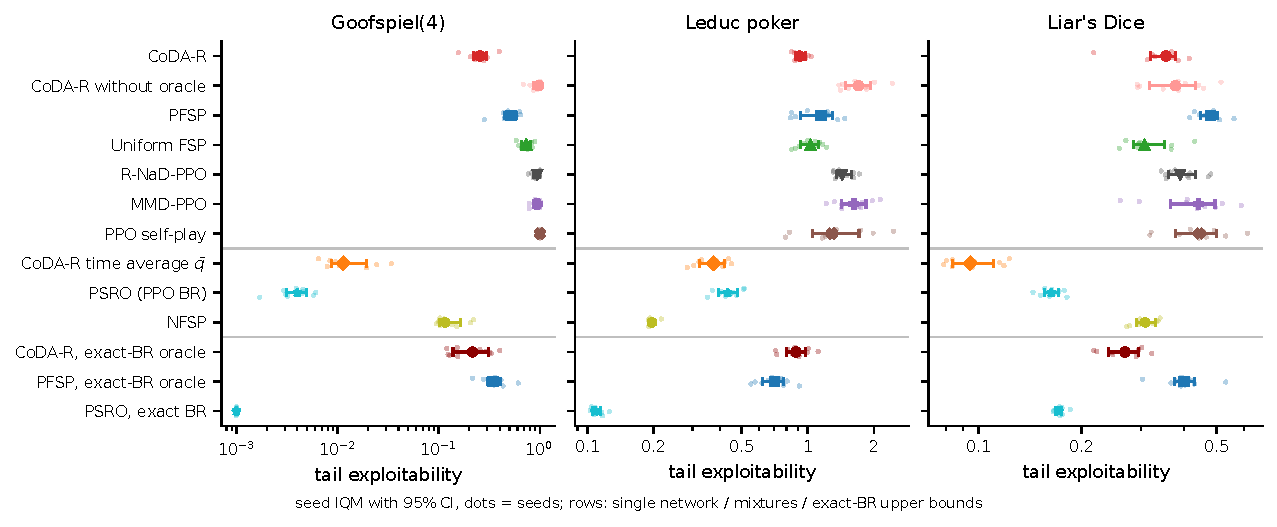
\includegraphics[width=0.9\linewidth]{figures/main_tail.pdf}
\end{center}
\caption{Tail exploitability per seed (dots) with IQM and 95\% CI, on a log scale. Rows: single networks, mixtures, and exact-BR controls.}
\label{fig:main-tail}
\end{figure}

\FloatBarrier
\subsection{Large Games}

Checkpoints are evaluated at the budget fractions $1/64$, $1/16$, $1/4$, $0.8$, $0.9$, and $1$ (Figure~\ref{fig:scale}). For the play against earlier checkpoints (Figure~\ref{fig:scale-history}), each run stores 16 checkpoints and every ordered pair plays 1000 sampled games with alternating seats. An earlier checkpoint counts as beaten when the later checkpoint's loss rate against it is at most 0.45, and as beating the later checkpoint when that loss rate is at least 0.55.

\begin{figure}[!htbp]
\begin{center}
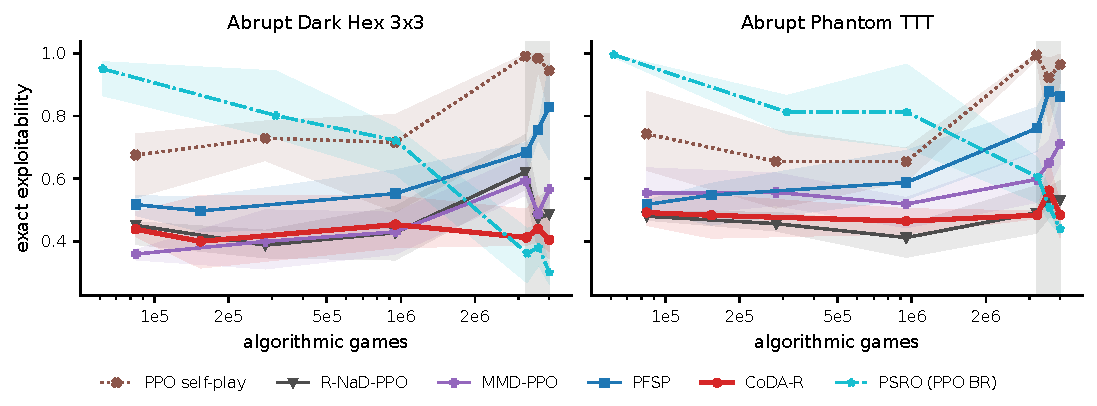
\includegraphics[width=0.85\linewidth]{figures/scale_curves.pdf}
\end{center}
\caption{Exact exploitability on the large games (seed mean and 95\% CI, 5 seeds). The gray band marks the tail.}
\label{fig:scale}
\end{figure}

\begin{figure}[!htbp]
\begin{center}
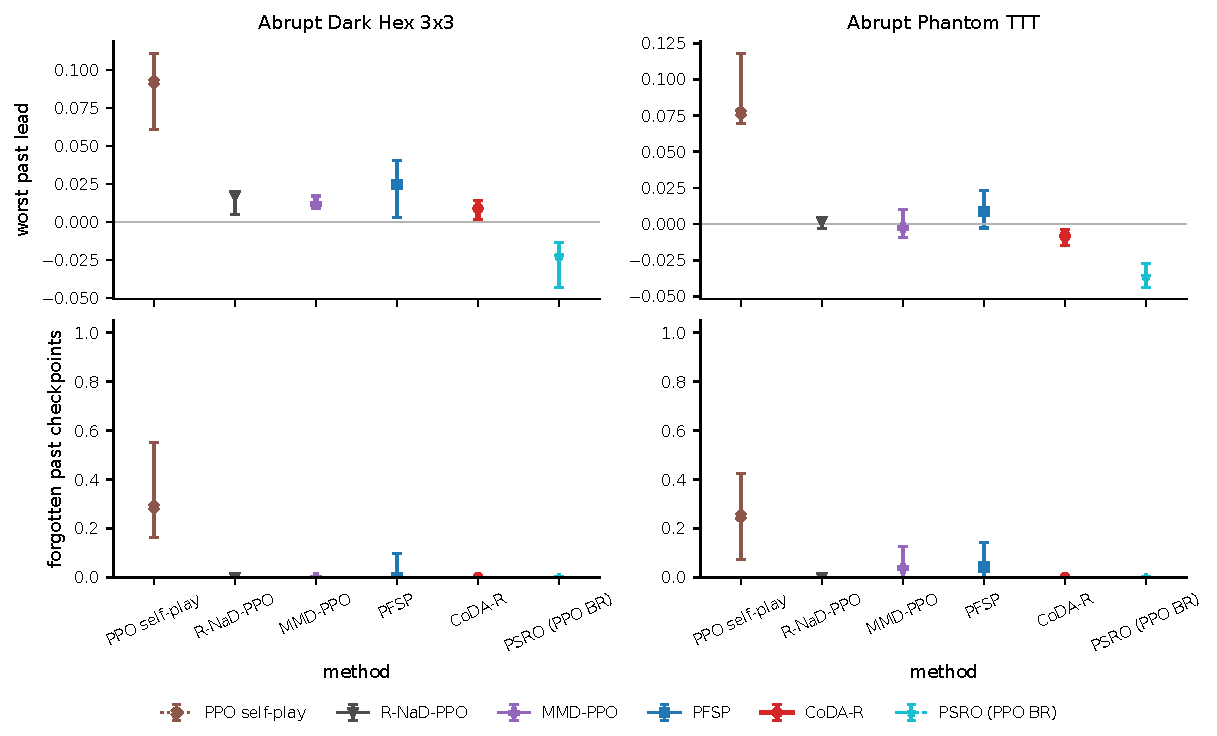
\includegraphics[width=0.85\linewidth]{figures/scale_history.pdf}
\end{center}
\caption{Play against one's own earlier checkpoints on the large games. Top: the worst lead of an earlier checkpoint over a later one, averaged over checkpoints. Bottom: the fraction of checkpoints that were once beaten and later beat a newer checkpoint.}
\label{fig:scale-history}
\end{figure}

\FloatBarrier
\subsection{What the Pool Buys}
\label{app:mech}

\textbf{Sleeper members.} The base network is \rnad{} trained for $2\times10^5$ games, the target member is its full-tree best response, and the three decoys are random networks. The pool follows the main protocol with the oracle switched off. After the reset, each branch trains for 96 more rollouts. Hedge and fixed mixing use the $\eta$ and entropy coefficient of \rnad{} with self-play share 0.5, and fixed mixing gives the target a coefficient of 0.35; the moving-anchor rule uses the configuration of \codar{}. The target counts as repaired when the learner's loss rate against it stays at most 0.52 for 3 consecutive rollouts (Table~\ref{tab:sleeper}, Figure~\ref{fig:sleeper}).

\begin{table}[!htbp]
\caption{Sleeper members: rollouts needed to repair the target again after the reset (IQM over 6 seeds; ``---'': not repaired within 96 rollouts) for suppression lengths $T=24/48/96/192$, and the share of the training weight held by members that do not beat the learner (range over $T$).}
\label{tab:sleeper}
\begin{center}
\footnotesize
\setlength{\tabcolsep}{4pt}
\begin{tabular}{lcccc}
\toprule
 & \multicolumn{2}{c}{Goofspiel(4)} & \multicolumn{2}{c}{Leduc poker} \\
Rule & repair time & idle weight & repair time & idle weight \\
\midrule
\codar{} & 1 / 1 / 1.2 / 1 & 0.006--0.015 & 3 / 5 / 5.8 / 4.2 & 0.11--0.13 \\
Moving dual anchor & 1 / 1 / 1.2 / 1 & 0.006--0.017 & 3 / 3.7 / 4 / 3.7 & 0.17--0.22 \\
PFSP & 1 / 2.3 / 1.5 / 1.5 & 0.49--0.50 & 7.5 / 13.2 / 11 / 14.3 & 0.46--0.47 \\
Uniform FSP & 8 / 14 / 19.3 / 14.5 & 0.10 & 19.5 / 40.3 / 37.5 / 40.4 & 0.17--0.18 \\
Hedge & 0.3 / 1.7 / 4.8 / 31.5 & 0.49--0.50 & 3.3 / 8 / 9.7 / 37.7 & 0.44--0.47 \\
Fixed mixing & 0 / 0 / 0.2 / 0 & 0.35 & 4 / 4.7 / 5.8 / 4.3 & 0.28--0.31 \\
\rnad{} (no pool) & 7.9 / 15.7 / 5.8 / 26.8 & --- & 50 / 48 / 79.5 / --- & --- \\
\bottomrule
\end{tabular}
\end{center}
\end{table}

\begin{figure}[!htbp]
\begin{center}
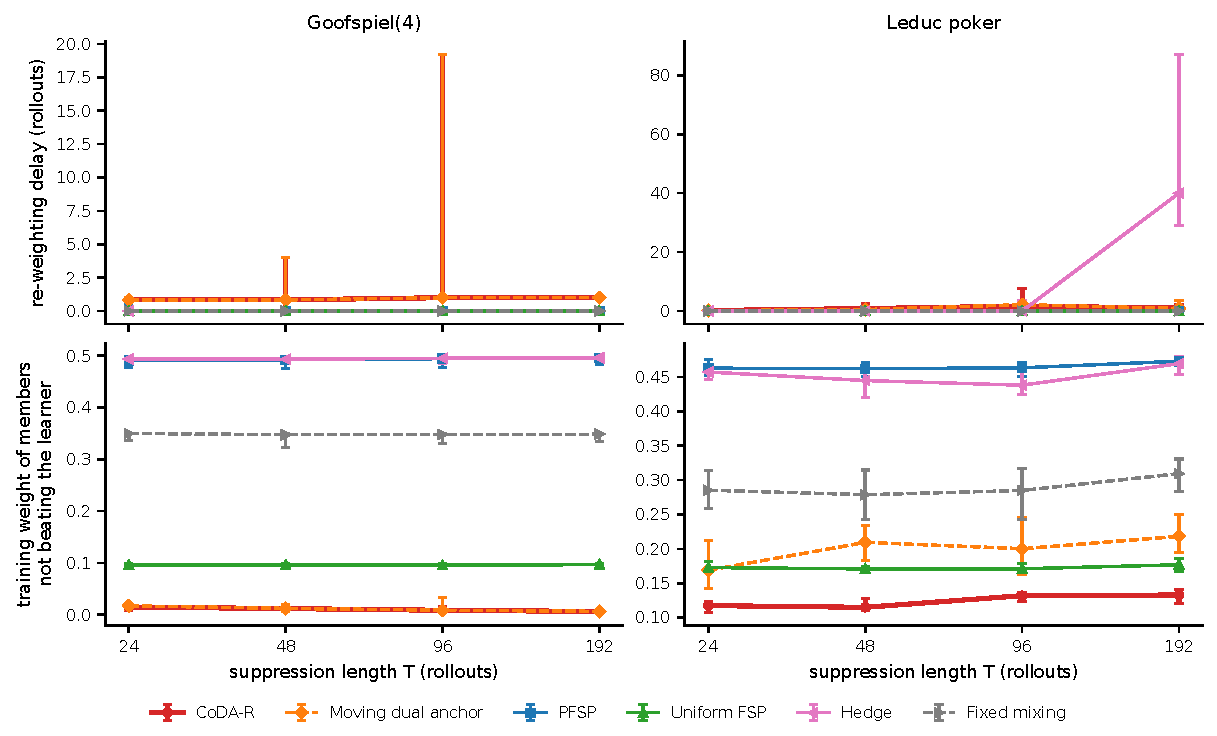
\includegraphics[width=0.8\linewidth]{figures/vuln_sleeper.pdf}
\end{center}
\caption{Sleeper members. Top: rollouts until the target regains half of the coefficient it had before the reset. Bottom: share of the training weight held by members that do not beat the learner.}
\label{fig:sleeper}
\end{figure}

\textbf{Hidden vulnerabilities.} The base is the average strategy of 2000 CFR+ iterations distilled into a network of the learner's size (maximum total variation 0.006--0.028 per information set). Each band holds up to 4 planted vulnerabilities, each at an information set that the learner reaches with probability at least 0.1 and where the planted action loses at least 0.05 in normalized score per visit. The pool holds only the exact best response to the damaged network, with the main protocol and the oracle switched off; \rnad{} only records its loss rate against the attacker. Each branch trains for 256 rollouts, and a vulnerability counts as repaired when the probability of the planted action stays at most 0.5 for 3 rollouts. The band $[0.3,1)$ on Leduc serves as a control, since its planted actions lose only 0.14 per visit and the attacker leads by 0.002 (Table~\ref{tab:hidden}).

\begin{table}[!htbp]
\caption{Hidden vulnerabilities: median rollouts to repair (seeds repaired out of 6) and mean coefficient of the attacker. ``$>256$'': median not repaired.}
\label{tab:hidden}
\begin{center}
\footnotesize
\begin{tabular}{llccc}
\toprule
Game & Opponent reach & \rnad{} (no pool) & PFSP & \codar{} \\
\midrule
Leduc & $[0.3,1)$ (control) & $>256$ (3) & $>256$ (2), 0.17 & $>256$ (3), 0.05 \\
Leduc & $[0.03,0.1)$ & 41.5 (6) & 19.5 (6), 0.16 & 30 (6), 0.04 \\
Leduc & $[0.003,0.01)$ & 232.5 (4) & 52 (5), 0.17 & 168.5 (4), 0.06 \\
Leduc & $[0,0.001)$ & $>256$ (0) & 8.5 (6), 0.17 & 21 (6), 0.03 \\
Goofspiel(4) & $[0.3,1)$ & 127.5 (6) & 159 (6), 0.35 & 132 (6), 0.67 \\
Goofspiel(4) & $[0,0.001)$ & $>256$ (0) & $>256$ (0), 0.05 & $>256$ (0), 0.002 \\
\bottomrule
\end{tabular}
\end{center}
\end{table}

\textbf{Retention.} The starting network is the same distilled CFR+ base without planted vulnerabilities. Each method trains for $10^6$ games under the main protocol, with its oracle where applicable, and with the entropy coefficient fixed at its tuned final value. Exploitability is measured every 16 rollouts. An archive receives a copy of the learner every 128 rollouts, starting with the base; it is used only for evaluation, identically for methods with and without a pool. An archived version counts as beaten when the learner's loss rate against it is at most 0.49, and as beating the learner again when that loss rate is at least 0.51. The drift loss is the per-visit loss in normalized score relative to the CFR+ base at information sets that the learner itself often reaches, grouped by the probability with which self-play opponents reach them (Table~\ref{tab:retention}, Figure~\ref{fig:drift}).

\begin{table}[!htbp]
\caption{Retention from a near-Nash start (IQM over 6 seeds): rise of the tail exploitability over the start, drift loss in the band with opponent reach below $10^{-3}$, and the fraction of archived versions that were once beaten and later beat the learner.}
\label{tab:retention}
\begin{center}
\footnotesize
\begin{tabular}{lcccccc}
\toprule
 & \multicolumn{3}{c}{Goofspiel(4), start $3.8\times10^{-4}$} & \multicolumn{3}{c}{Leduc poker, start 0.0088} \\
Method & rise & drift & forgotten & rise & drift & forgotten \\
\midrule
PPO self-play & 1.000 & 0.0556 & 0 & 1.642 & 0.0157 & 0.229 \\
\rnad{} & 0.979 & 0.0150 & 0 & 1.353 & 0.0093 & 0 \\
MMD-PPO & 0.884 & 0.0144 & 0 & 1.316 & 0.0111 & 0.063 \\
PFSP & 0.275 & 0.0017 & 0 & 1.514 & 0.0040 & 0 \\
\codar{} & 0.135 & 0.0074 & 0 & 1.189 & 0.0030 & 0 \\
\codar{}, $c\times0.5$ & 0.177 & 0.0046 & 0 & 1.227 & 0.0029 & 0 \\
\codar{}, $c\times2$ & 0.218 & 0.0134 & 0 & 1.182 & 0.0031 & 0 \\
\bottomrule
\end{tabular}
\end{center}
\end{table}

\begin{figure}[!htbp]
\begin{center}
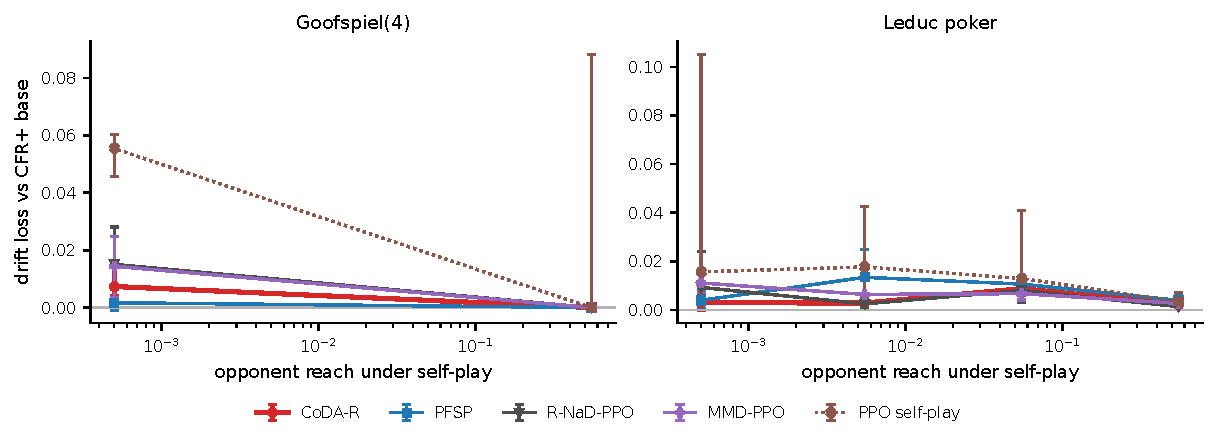
\includegraphics[width=0.8\linewidth]{figures/forgetting_drift.pdf}
\end{center}
\caption{Retention: drift loss relative to the CFR+ base against the probability with which self-play opponents reach the information set (IQM and 95\% CI, 6 seeds). On Goofspiel(4) only the highest and lowest bands contain information sets.}
\label{fig:drift}
\end{figure}

\textbf{Open pools.} The members are, in order, the average strategies of CFR+ after 3 and 30 iterations, two legacy agents with $2\times32$ networks, two scripted bots, and the uniform policy, followed by alternating random networks and duplicates up to $N$ members. There is no oracle and no snapshot, and the budget is $10^6$ games (Figure~\ref{fig:open-pool}).

\begin{figure}[!htbp]
\begin{center}
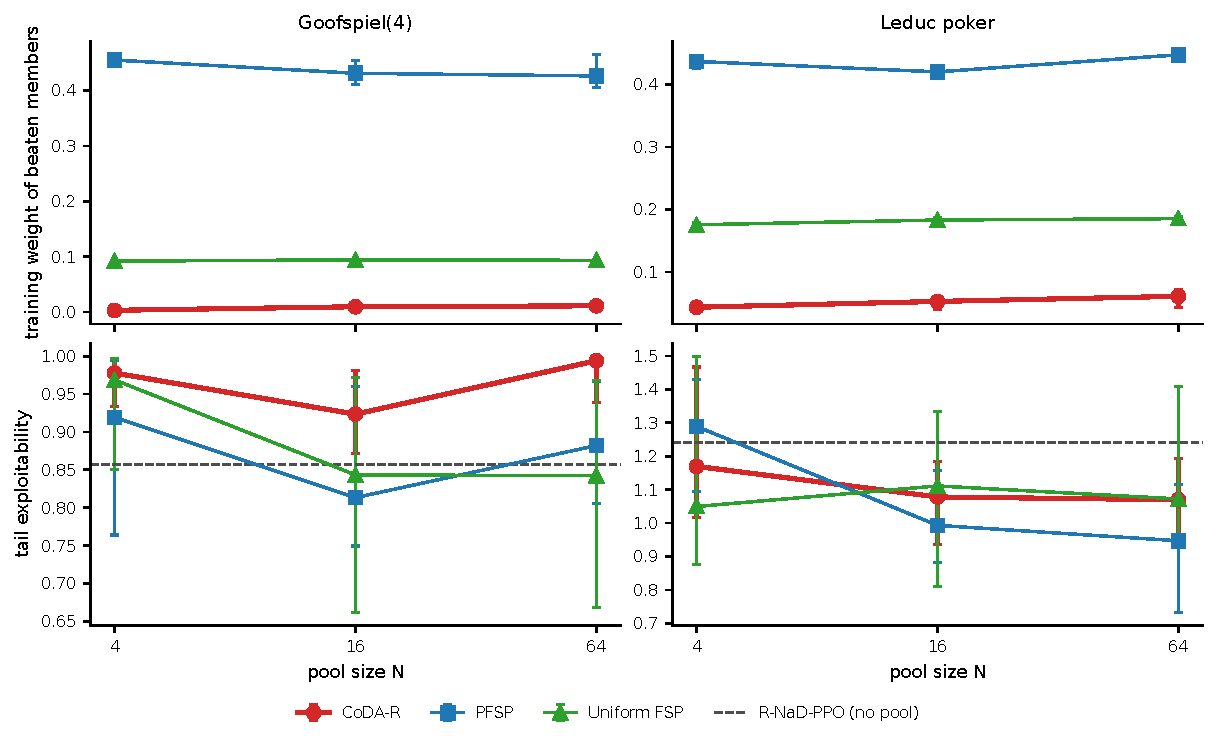
\includegraphics[width=0.8\linewidth]{figures/open_pool.pdf}
\end{center}
\caption{Open pools of $N$ external members. Top: share of the training weight held by members that the learner already beats. Bottom: tail exploitability (IQM and 95\% CI, 6 seeds); the dashed line is \rnad{} without a pool.}
\label{fig:open-pool}
\end{figure}

\FloatBarrier
\subsection{Ablations}

On Leduc, a pool capacity of 16 coincides with the base configuration, because the pool never fills 8 slots there (Figure~\ref{fig:ablations}).

\begin{figure}[!htbp]
\begin{center}
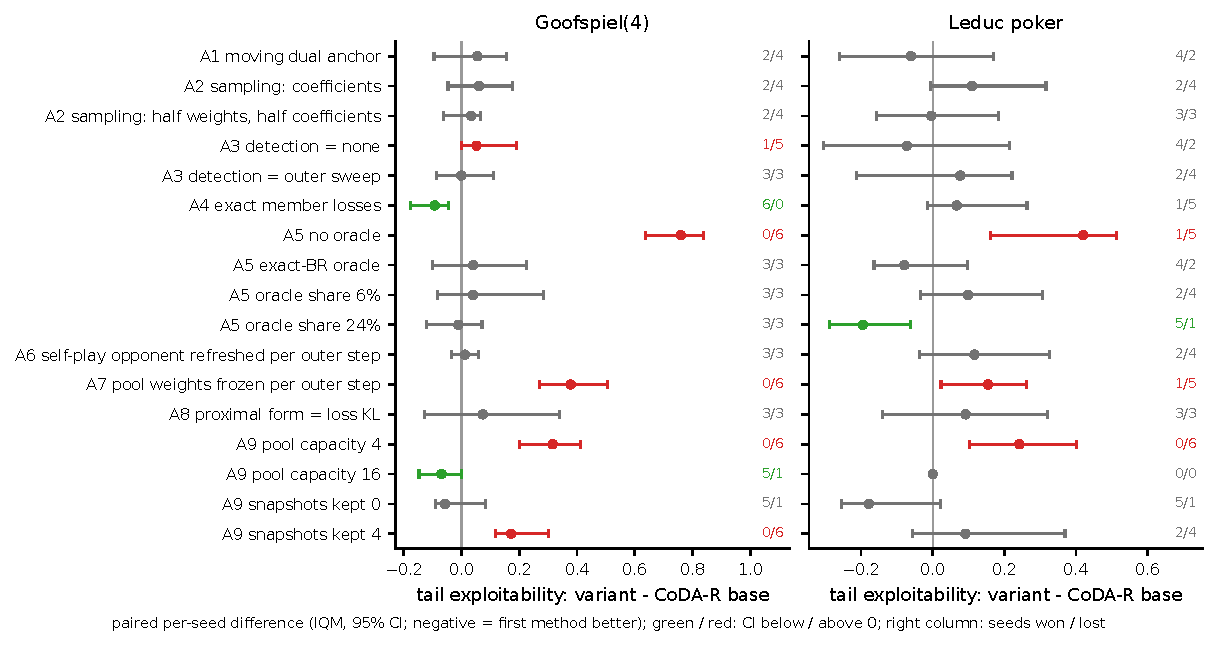
\includegraphics[width=0.9\linewidth]{figures/ablations_forest.pdf}
\end{center}
\caption{Ablations ($10^6$ games, 6 seeds): per-seed paired difference in tail exploitability, variant minus base (IQM and 95\% CI; negative is better), with the seeds won and lost.}
\label{fig:ablations}
\end{figure}

\FloatBarrier
\subsection{The Exact Algorithm on Matrix Games}
\label{app:theory-figs}

The checks of \S\ref{sec:exp-theory} cover 1406 experimental cells and all inequalities of \S\ref{sec:theory}: the energy inequality, the certificates, the rates, the mixtures, the versions with injected errors $\xi$ and $\delta$, and Theorem~\ref{thm:oracle}. In Figure~\ref{fig:oracle-rate}, each step adds the exact best response to the policy anchor to the pool, which keeps the last 8 members; the dual strength is $c=\min(4,2\eta/\|S\|^2)$, the largest value that Theorem~\ref{thm:oracle} allows, and the approximate oracle has error $\varepsilon=0.01$. In Figure~\ref{fig:basin}, each cell has 200 random starts, and game sizes, pool sizes, and $\eta$ are pooled. The adversarial pools of Figure~\ref{fig:adversarial} are periodic best responses (benign), the reflection of the learner about the Nash point (complement), many random strategies (flood), the pure strategies on the Nash support, which always tie (support), and best responses to long-past iterates (stale). In Figure~\ref{fig:pool-rules}, the rules with a fixed share (PFSP, uniform, Hedge) stall between $10^{-2}$ and $6\times10^{-2}$ because tied members keep their share, while \codar{} and the empty pool reach $10^{-11}$ before and after the reset. In Figure~\ref{fig:inexact}, the final exploitability scales with $\delta$, as in the bounded-error case of Theorem~\ref{thm:inexact}, and the estimation error matters only when the pool is non-empty and $\delta=0$.
\begin{figure}[!htbp]
\begin{center}
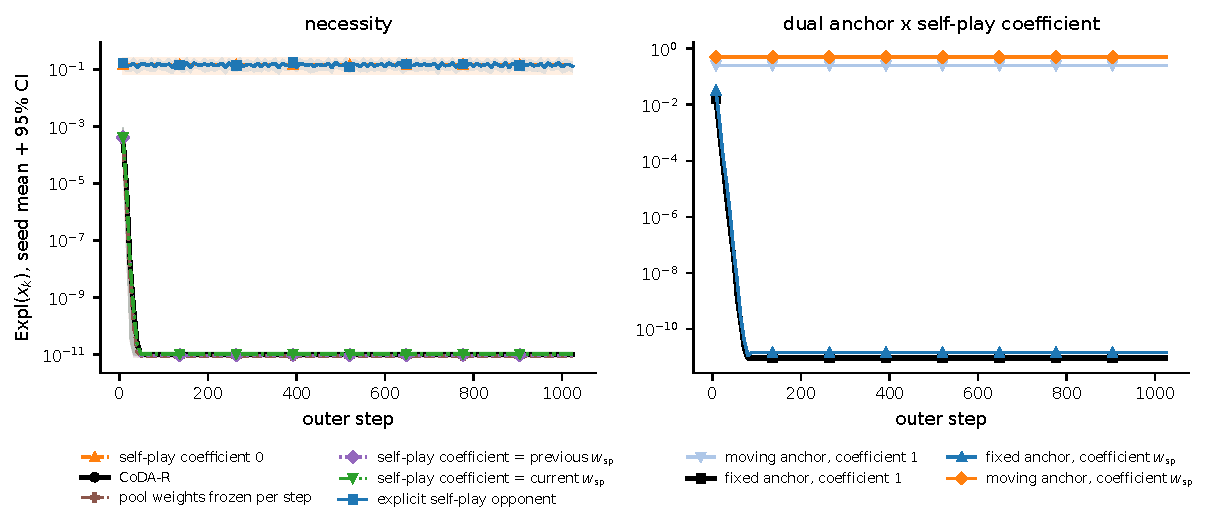
\includegraphics[width=0.85\linewidth]{figures/theory_necessity.pdf}
\end{center}
\caption{Necessity of the design elements (seed mean and 95\% CI of exploitability). Left: explicit self-play opponent, other self-play coefficients, and frozen pool weights. Right: fixed and moving dual anchor, started at the fixed point of Proposition~\ref{prop:rps}.}
\label{fig:theory-nec}
\end{figure}

\begin{figure}[!htbp]
\begin{center}
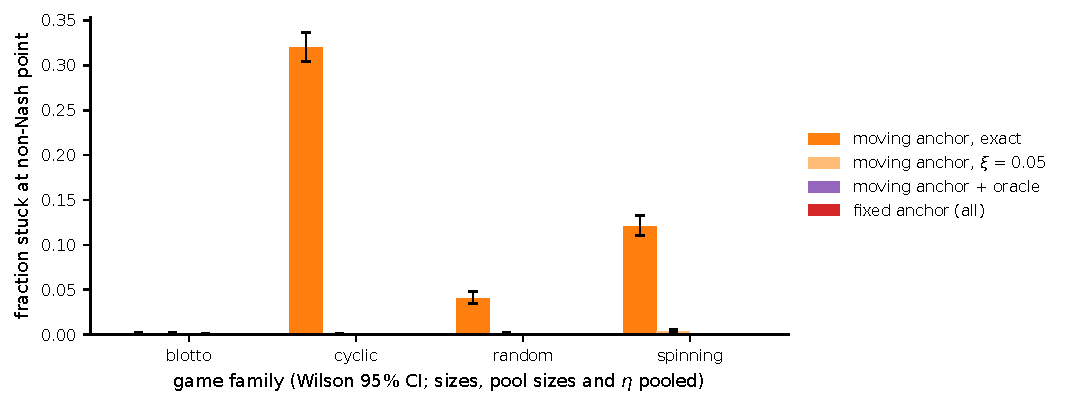
\includegraphics[width=0.75\linewidth]{figures/theory_anchor_basin.pdf}
\end{center}
\caption{Fraction of random starts from which the moving anchor gets stuck at a non-Nash point (Wilson 95\% CI). The fixed anchor never gets stuck.}
\label{fig:basin}
\end{figure}

\begin{figure}[!htbp]
\begin{center}
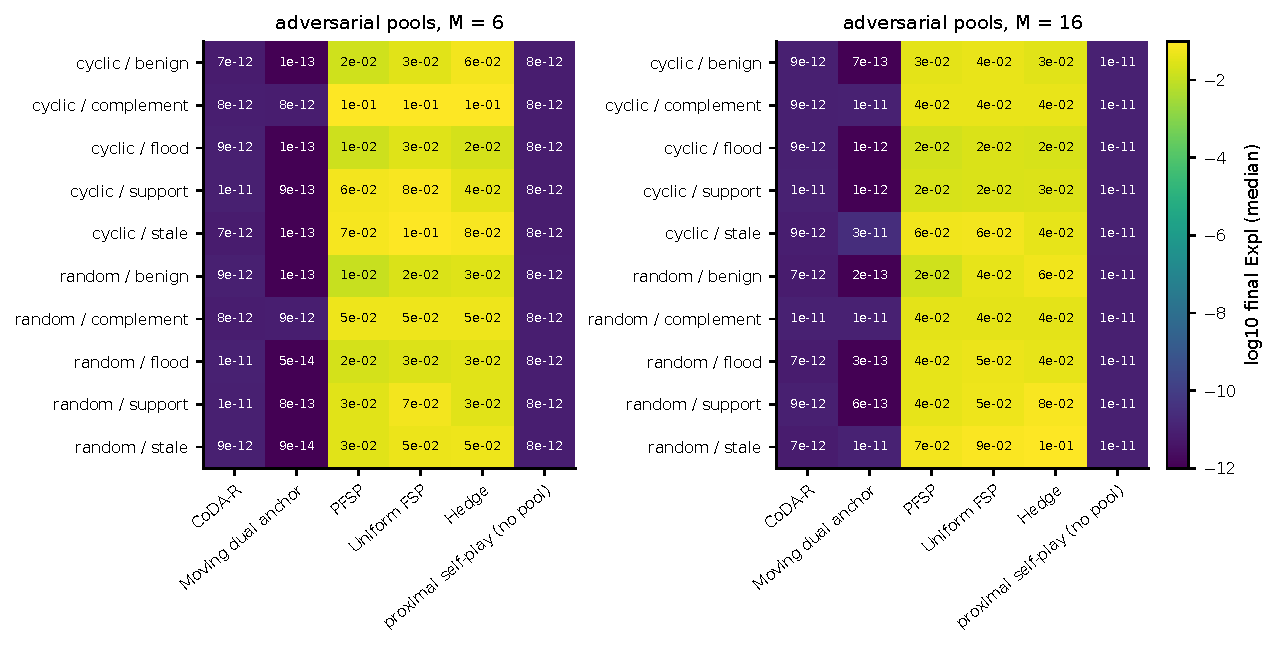
\includegraphics[width=0.9\linewidth]{figures/theory_adversarial_pool.pdf}
\end{center}
\caption{Adversarial pools: median final exploitability when an adversary chooses the pool members.}
\label{fig:adversarial}
\end{figure}

\begin{figure}[!htbp]
\begin{center}
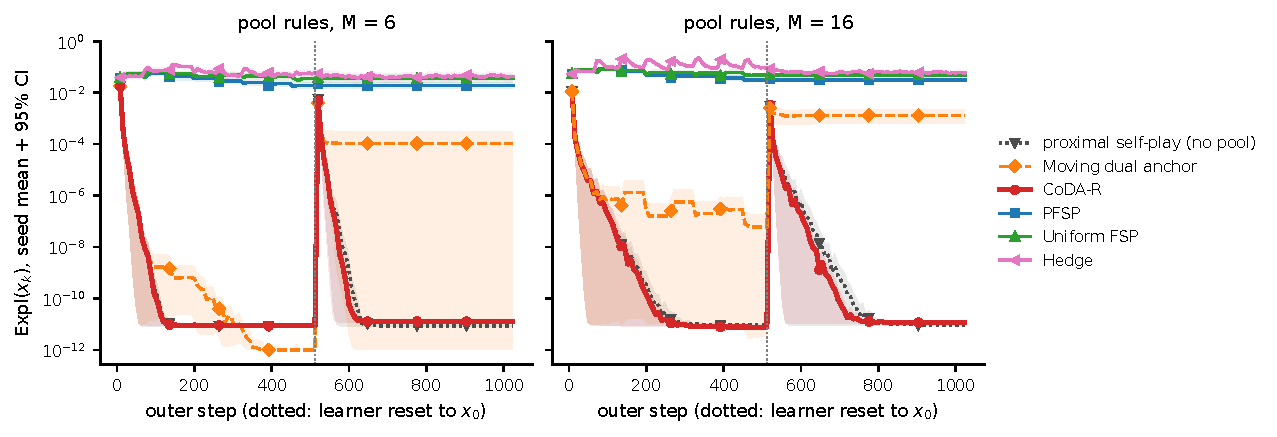
\includegraphics[width=0.9\linewidth]{figures/theory_pool_rules.pdf}
\end{center}
\caption{Pool rules on the same sequence of pools; at the dotted line, the learner is reset to its initial point.}
\label{fig:pool-rules}
\end{figure}

\begin{figure}[!htbp]
\begin{center}
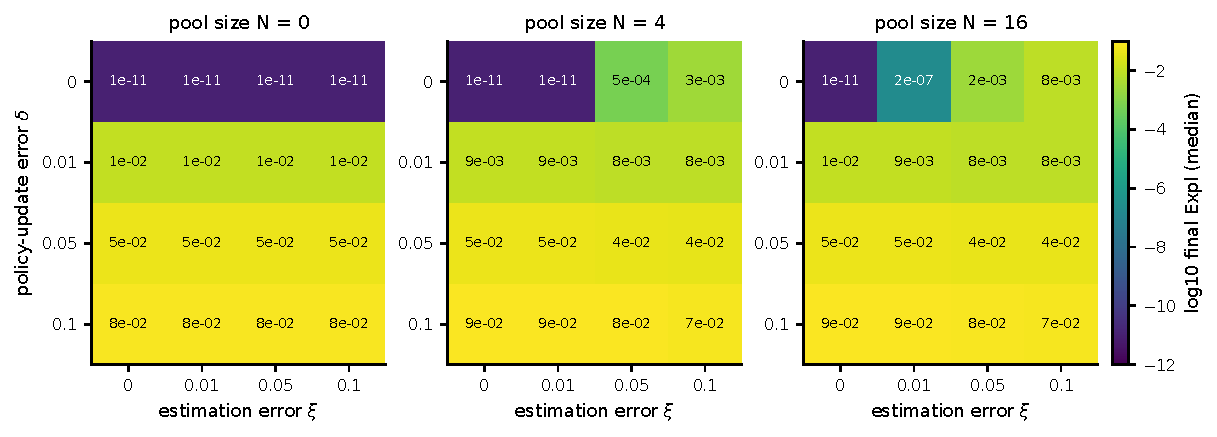
\includegraphics[width=0.85\linewidth]{figures/theory_inexact.pdf}
\end{center}
\caption{Injected errors: median final exploitability against the estimation error $\xi$ and the policy-update error $\delta$.}
\label{fig:inexact}
\end{figure}

\end{document}

